%%%%%%%%%%%%%%%%%%%%%%% file template.tex %%%%%%%%%%%%%%%%%%%%%%%%%
%
% This is a template file for The European Physical Journal
%
% Copy it to a new file with a new name and use it as the basis
% for your article
%
%%%%%%%%%%%%%%%%%%%%%%%% Springer-Verlag %%%%%%%%%%%%%%%%%%%%%%%%%%
%
% \begin{filecontents}{leer.eps}
% %!PS-Adobe-2.0 EPSF-2.0
% %%CreationDate: Mon Jul 13 16:51:17 1992
% %%DocumentFonts: (atend)
% %%Pages: 0 1
% %%BoundingBox: 72 31 601 342
% %%EndComments
% 
% % gsave
% % 72 31 moveto
% % 72 342 lineto
% % 601 342 lineto
% % 601 31 lineto
% % 72 31 lineto
% % showpage
% % grestore
% %%Trailer
% %%DocumentFonts: Helvetica
% \end{filecontents}
% %
% \documentclass[epj]{svjour}
% % Remove option referee for final version
% %
% % Remove any % below to load the required packages
% %\usepackage{latexsym}
% \usepackage{graphics}
% \usepackage{lineno,hyperref}
% \usepackage{graphicx}
% \usepackage{url}
% \usepackage{float}
% \usepackage{latexsym}
% \usepackage{amsmath,amssymb}
% \usepackage{dcolumn}
% \usepackage{epsfig}
% \usepackage{textcomp}
% \usepackage{multirow}
% \usepackage{soul}
% \usepackage{color}
% \usepackage{todo}
% \usepackage{adjustbox}
% \modulolinenumbers[5]
% % etc
% %
% \begin{document}
%
% \title{Time series analysis of temporal networks}
% %\subtitle{Do you have a subtitle?\\ If so, write it here}
% \author{Sandipan Sikdar\inst{1} \, Niloy Ganguly\inst{1} \and Animesh Mukherjee\inst{1}% etc
% % \thanks is optional - remove next line if not needed
% %\thanks{\emph{Present address:} Insert the address here if needed}%
% }                     % Do not remove
% %
% \offprints{}          % Insert a name or remove this line
% %
% \institute{\inst{1}Indian Institute of Technology Kharagpur, Kharagpur, India}
% %
% \date{Received: date / Revised version: date}
% % The correct dates will be entered by Springer
% %
% \abstract{
% A common but an important feature of all real-world
% networks is that they are temporal in nature, i.e., the network structure changes over time.
% Due to this dynamic nature, it becomes difficult to propose suitable growth models 
% that can explain the various important characteristic properties of these networks. 
% In fact, in many application oriented studies only knowing these properties is sufficient. For instance, if one wishes to launch a targeted attack on a network, 
% this can be done even without the knowledge of the full network structure; rather an estimate of some of the properties is sufficient enough to launch the attack.
% We, in this paper show that even if the network structure at a future time point is not available one can still manage to estimate its properties.
% We propose a novel method to map a temporal network to a set of time series instances, 
% analyze them and using a standard forecast model of time series, 
% try to predict the properties of a temporal network at a later time instance. To our aim, we consider 
% eight properties such as number of active nodes, average degree, clustering coefficient etc. and apply our prediction framework on them. 
% We mainly focus on the temporal network of human face-to-face contacts and observe that 
% it represents a 
% stochastic process with memory that can be modeled as Auto-Regressive-Integrated-Moving-Average (ARIMA). 
% We use 
% cross validation techniques to find the percentage accuracy of our predictions. 
% \textcolor{blue}{An important observation is that the frequency domain properties of the time series obtained from spectrogram analysis could be used to refine the 
% prediction framework by identifying beforehand the cases where the error in prediction is likely to be 
%  high. This leads to an improvement of {\bf 7.96\%} (for error level $\leq 20\%$) in prediction accuracy on an average across all datsets.}
%  %\todo{How much improvement - please write} 
% As an application we show how such prediction scheme can be used to launch targeted attacks on temporal networks.
% %
% \PACS{
%       {PACS}{89.75.Hc,89.75.Fb}   
% %       {89.75.Fb}
%      } % end of PACS codes
% } %end of abstract
% %
% \maketitle

\chapter{Analyzing structural properties of temporal networks}
This chapter is devoted to out first objective - understanding and predicting structural properties of temporal networks.

\noindent
\section{Introduction}
\label{introduction}
\if{0}
Recently the research community is reaching a consensus that many real 
networks have nodes and edges entering or leaving the system dynamically, thus making temporal networks a better way of representing these networks. 
Initial studies on temporal networks have been performed by aggregating the nodes and edges over all time 
steps and then analyzing the behavior of the aggregated network. This strategy however hides the time ordering of the nodes and the edges 
which may have a significant role in the understanding of 
the true nature of such temporal networks.
Researchers have subsequently come up with growth models and have proposed several metrics. Tang et al. have showed in ~\cite{TSMML10:smallworld} 
the presence of correlation and small world 
behavior in temporal networks. In ~\cite{stehle2010dynamical} the temporal network of human communication has been identified to be bursty in nature.
\fi
Understanding the structural properties of temporal network is of primary importance. To this end the research community was initially inclined towards 
aggregating the nodes and edges over all time 
steps and then analyzing the behavior of the aggregated network. This strategy however was found to hide the time ordering of the nodes and the edges 
which plays a significant role in understanding  
the true nature of such temporal networks. 
%This led researchers to come up with various growth 
% To the best of our knowledge no work has been done which provides a time series analysis of temporal networks in both 
% time and frequency domains. 
%In ~\cite{shimada2012networks} Shimada et al. propose a framework for transforming a static complex network to a time series using classical multi-dimensional scaling.
Recently, new network applications have cropped up where an estimate of the network properties are helpful even though the network structure is itself unavailable. 
For instance, in order to launch a targeted attack on the network one might not require the full knowledge of the network structure. Instead, an approximate estimate of some 
of the properties might be useful in finding the order in which the nodes and the edges may be removed. 

In this work, 
we propose a simple strategy to represent a temporal network as time series. Essentially, we consider a temporal network as a set of static snapshots collected 
at consecutive time intervals and represent each of them in terms of the properties of the network. In specific, we consider eight properties namely number of 
active nodes, average degree, clustering coefficient, number of active edges, betweenness centrality, closeness 
centrality, modularity and edge-emergence ~\cite{sur2014attack}. 
%Note that this framework serves as a remarkable handle for transforming a network analysis problem to a classical time series analysis problem. Indeed

We then use the known analytical tools for time series predictions to predict the network properties at a future time instance. 
Note that the time series framework can be particularly effective as it is impossible to 
define a unified network evolution/growth model for temporal networks simply because the  
rules of temporality are varied across systems. Hence the feasible alternative could be to learn 
the evolution pattern (which we do through time-series analysis) and then predict the later time steps. 

Due to various irregularities in the time series, predictions at certain points are erroneous. Therefore we 
further refine our prediction framework using spectrogram analysis by identifying beforehand the cases where the 
prediction error is high i.e., unsuitable for prediction. In fact we observe that the accuracy of the framework is 
enhanced further by 7.96 (for error level $\leq 20\%$) on an average across all datasets 
if we remove 
the cases which are deemed unsuitable for prediction by spectrogram analysis.

As an application we also propose a strategy to launch targeted attacks based on our prediction framework and show that this scheme beats the state-of-the-art ranking method 
used for such attacks. We believe that our framework could be used in designing ranking schemes for nodes in temporal networks at a future time step  
albeit the network structure at that time step itself is unknown.
%\textcolor{blue} {%In particular, 
% We perform our experiments on two types of human face-to-face communication network, 
% we observe that the properties could be segregated based on time domain and frequency domain analysis 

%  As an additional objective, we perform frequency domain 
%  analysis of these time series in order to enrich our predictions. 
%We use three types of data sources for our experiments: (i) time-varying human face-to-face interaction networks, (ii) Twitter hashtag co-occurrence graph 
%varying over the period of an event (e,g., London Olympics) and (iii) Facebook posts graph of a set of users. 

%\todo{This paragraph needs to be discussed}
%We report our prediction results on real world time-varying networks. 
We perform our experiments on five different human face-to-face communication networks 
and observe that the above properties could be segregated based on time domain and frequency domain (spectrogram) characteristics. 
In general this method allows us to make predictions with very low errors.   
 Importantly, the frequency domain analysis also nicely separates out those properties that can be predicted with low errors from those for which it is not 
 possible.
\if{0} 
Rest of the paper is organized as follows. In Section ~\ref{relatedworks} we present a brief review of the literature. 
Section ~\ref{mapping} describes the framework for mapping temporal networks to time series. 
Section ~\ref{dataset} provides a brief description of the datasets we use for 
our experiments.
  In section ~\ref{properties} we perform a detailed time domain and frequency domain analysis of the time series. 
Section ~\ref{prediction} outlines the description of our prediction framework. In Section ~\ref{result} we provide the detailed results of our prediction framework on the 
human face-to-face communication networks. We also show how the prediction scheme could be enhanced using the spectrogram analysis. We further 
propose an attack strategy based on the prediction scheme and show that it beats the state-of-the-art methods (section ~\ref{attack}). 
We conclude in section ~\ref{conclusion} by summarizing our main contributions and pointing to certain future directions.
\fi
\medskip


%\noindent
\section{Related works}
\label{relatedworks}
Most of the initial works attempted to study temporal networks by aggregating the network across all times and then analyzing this aggregated network.
However, it was found that
time ordering is an important issue and destroying this ordering information severely affects the understanding of the true nature of the network. 
Several ways have been therefore devised to represent temporal networks. Basu et al. 
have shown in ~\cite{journals/corr/abs-1012-0260} a way of representing temporal networks as a time series of static graph snapshots and have proposed a stochastic model for generating 
temporal networks. Perra et al. in ~\cite{perra2012activity} have provided an activity driven modeling of temporal networks. They define activity potential which is a time 
invariant function characterizing the agents' interactions and propose a formal model of temporal networks based on this idea. Random walks have been introduced in 
temporal networks ~\cite{starnini2012random} to single out the role of the different properties of the empirical networks. It has also been shown that random walk 
exploration is slower on temporal networks than it is on the aggregate projected network. Several other modeling frameworks for temporal networks have also 
been proposed (see ~\cite{vespignani2011modelling,hill2010dynamic,hanneke2010discrete} for references). Apart from the attempts to generate temporal networks several other properties of these networks have also been investigated.
Temporal networks of human communication has been observed to be bursty in nature in ~\cite{barabasi2005origin}. Dynamics of human face-to-face interactions have been studied in ~\cite{zhao2011social}.
~\cite{tang2009temporal} shows how the presence of burstiness affects the dynamics of diffusion process. Further different metrics to study the properties of temporal networks 
have also been proposed in ~\cite{pan2011path}.  

On the other hand, time series have found a lot of applications in economic 
analysis and financial forecasting ~\cite{hamilton1989new}. It has also been applied in tweet analysis ~\cite{o2010tweets}. 
However, temporal networks have not 
been studied in details so far as a time series problem except for preliminary attempts in ~\cite{scherrer2008description,hempel2011inner}.
\textcolor{blue}{In ~\cite{scherrer2008description} the authors analyze temporal networks as time series but to the best of our knowledge this is the first 
work which leverages the time series forecasting tools to predict the network properties at a future time instant. 
Frequency domain analysis on the time series representing 
temporal network and its implication also remain unexplored to the best of our knowledge.}
 Therefore we propose to leverage in this paper the standard 
techniques of time series analysis (both in time and frequency domain) to understand the dynamical properties of temporal networks.
Our prime contribution is to develop a unified framework to analyze and predict different properties of temporal networks based on time-series modeling.

\medskip


\noindent
\section{Mapping Temporal network to time series}
\label{mapping}
%In this section we describe how we transform a temporal network to a set of time series representing it. 

\begin{figure}
 \begin{center}
 \includegraphics*[width=0.7\columnwidth, angle=0]{./texfiles/Chapter_1/fig/Presentation_d-eps-converted-to.pdf}
 \caption{\label{fig1}Converting Temporal network to Time series}
 \end{center}
 \end{figure}

 We consider a temporal network as a set of static snapshots collected at consecutive time intervals. 
%In this way a temporal graph can be represented as series of static graphs. 
Each snapshot is then represented in terms of eight (mainly structural) properties of the underlying graph. 
 Consequently we obtain a set of points ordered in time or equivalently a discrete time series (see figure ~\ref{fig1}). 
The eight properties we use to represent the temporal network as a time series are:
 
 \begin{itemize} 
  \item (1). {\bf  Number of active nodes}: This is the count of the number of nodes in the system at a given time step. We consider active nodes to be those which have non-zero degree in a time step. We represent the number of active nodes in the system at time step {$t$} by {$N_{t}$}.
  In a similar way we define (2). {\bf number of active edges} and (3). {\bf average degree} and represent the values of these properties at time $t$ by $E_t$ and $Avg\_deg_{t}$ respectively.
  %\item {\bf Average degree}: This is the average degree of the network snapshot at a given time step. We represent average degree at time instance {\large$t$} by 
  %{$Avg\_deg_{t}$}. 
  %\begin{center}
   %{$Avg\_deg_{t}$}={$\frac{2 \times E_{t}}{N_{t}}$}
  %\end{center}

%   \item {\bf Betweenness centrality}: Betweenness centrality of a node is 
%   equal to the number of shortest paths from all vertices to all others that pass through that node.
%   We measure betweenness centrality, represented by {$Bet\_cen_{t}$} of the network snapshot at a given time step {$t$} as the average of the 
%   the betweenness centrality values of the active nodes in the network at $t$.
%   \item {\bf Closeness centrality}: Closeness centrality of a node is the mean distance of that node to all other nodes in the network. 
%     We measure closeness centrality, represented by {$Clos\_cen_{t}$} of the network snapshot at a given time step {$t$} as the average of the 
%   the closeness centrality values of the active nodes in the network at $t$.
%   \item {\bf Clustering coefficient}: We calculate the average clustering coefficient of the active nodes
%   of the network snapshot at a given time step. We represent the average clustering 
%   coefficient at a given time step {$t$} by {$Cluster\_coeff_{t}$}.
\begin{figure}[h]
 \begin{center}
 
 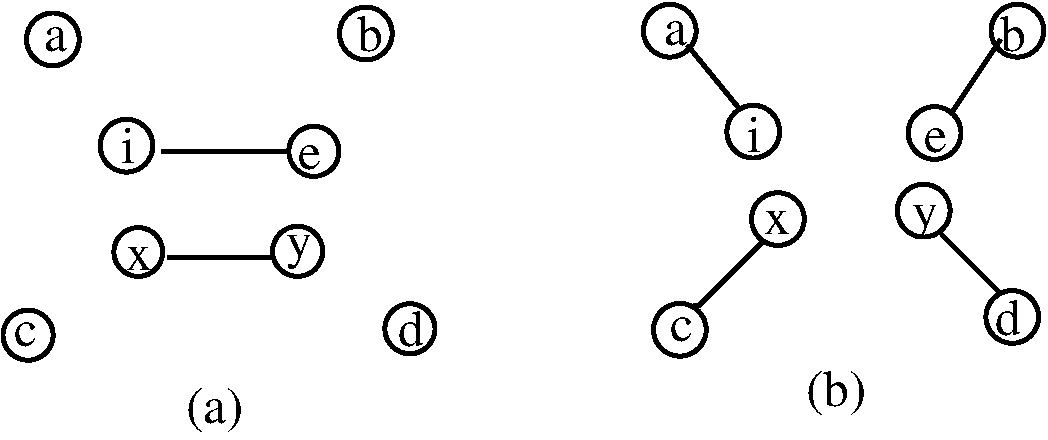
\includegraphics[width=0.7\columnwidth, angle=0]{./texfiles/Chapter_1/fig/ede_em-eps-converted-to.pdf}
 \caption{\label{fig3}(a) and (b) denote the status of the network at time $t$ and $t+1$ respectively. For the edge $(i,e)$ in $t$ the corresponding edges
 emanating from $i$ and $e$ are $(i,a)$ and $(e,b)$. For the edge $(x,y)$ they are $(x,c)$ and $(y,d)$. So the $Edge\_emer_{t}=\frac{2+2}{2}=\frac{4}{2}$}
 
%  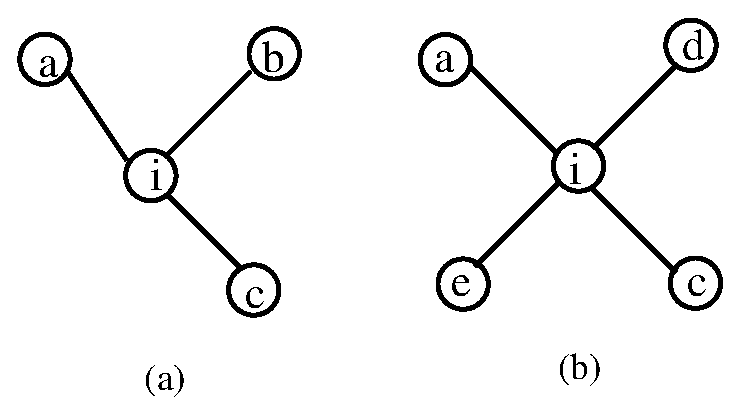
\includegraphics[width=0.8\columnwidth, angle=0]{fig/jaccard.eps}
%  \caption{\label{fig2}(a) and (b) denote the status of node $i$ at time $t$ and $t+k$ respectively. $NBR(i)_{t}=\{a,b,c\}$ and $NBR(i)_{t+k}=\{a,d,c,e\}$ 
%  $Correlation(i)_{k}$={\large$\frac{NBR(i)_{t}\bigcap NBR(i)_{t+k}}{NBR(i)_{t}\bigcup NBR(i)_{t+k}}$}={\large$\frac{2}{5}$} where $NBR(i)_{t}\rightarrow$ the set of neighbors of $i$ at time $t$}
%   
%    \includegraphics[width=0.9\columnwidth, angle=0]{fig/aging_inf2006.eps}
%  \caption{\label{aging}The value of the correlation decreases as we increase the lag between the network snapshots (INFOCOM 2006 dataset). The $X$ axis represents lag and $Y$ axis
%   represents the average correlation value.\vspace{-6mm}}
  
 
 \end{center}
 \end{figure}

   
\item (4). {\bf  Edge emergence}: Edge emergence ~\cite{sur2014attack} is a measure that estimates structural similarity. For measuring the 
  edge emergence at time $t$ we consider each edge of the network at time $t$ and for each of its two endpoints we calculate the number of edges 
  emerging in the next time step $t+1$. We represent edge-emergence at time $t$ by $Edge\_emg_{t}$. If $E_t$ denotes the set of edges present in the network at time $t$ 
  and $A_{t+1}$ denotes the set of edges at time $t+1$ which are adjacent to $E_t$ then $Edge\_emg_{t}=\frac{|A_{t+1}|}{|E_{t}|}$. 
Figure~\ref{fig3} shows how we calculate this measure for a temporal network at any time instance.
  
  
  \item (5). {\bf  Modularity}: We decompose each snapshot into communities using the technique specified in ~\cite{blondel2008fast}
  and measure the goodness of this division using modularity ~\cite{newman2006modularity}. We represent modularity 
  of the system at a given time step {$t$} by {$Mod_{t}$}. 
  
%   We also consider {\bf betweenness centrality}, {\bf closeness centrality} and {\bf clustering coefficient} and their values at time step $t$ are represented by 
%   {$Bet\_cen_{t}$}, {$Clos\_cen_{t}$} and {$Cluster\_coeff_{t}$} respectively.
  
 \end{itemize}
 We also consider (6). {\bf  betweenness centrality}, (7). {\bf closeness centrality} and (8). {\bf  clustering coefficient} of the graph (values computed for each node and then summed over all nodes) 
and their values at time step $t$ are represented by 
  {$Bet\_cen_{t}$}, {$Clos\_cen_{t}$} and {$Clus\_coeff_{t}$} respectively.

\medskip


\noindent
\section{Description of the dataset}
\label{dataset}
We perform our experiments on five human face-to-face network datasets: INFOCOM 2006 dataset~\cite{cambridge-haggle-imote-infocom2006-2009-05-29}, SIGCOMM 2009 dataset~\cite{thlab-sigcomm2009-mobiclique-proximity-2012-07-15}\footnote{http://crawdad.org/}, 
Highschool datasets (2011, 2012)~\cite{fournet2014contact} and Hospital dataset~\cite{vanhems2013estimating}\footnote{http://www.sociopatterns.org/}.


% \textcolor{blue}{The first two represent human face-to-face interaction while the last two represent 
% human interaction through social media.}
\begin{itemize}
\item {\bf INFOCOM 2006:}
This is a human face-to-face communication network and was collected at the IEEE INFOCOM 2006 conference at Barcelona.
78 researchers and students participated in the experiment. They were equipped with imotes and apart from them 20 stationary imotes were deployed as 
location anchors. The stationary imotes had more powerful battery and had a radio range of about 100 meters. The dynamic imotes had a radio range of 30 meters.
If two imotes came in each others' range and stayed for at least 20 seconds then an edge was recorded between the two imotes.
The edges were recorded at every 20 seconds. 
Therefore, this is the lowest resolution at which the experiments can be potentially conducted. However, we observe that at this resolution the network is extremely sparse 
which makes it difficult to conduct meaningful data comparison and prediction. We observe experimentally that the lowest interval that allows for appropriate comparison 
and prediction is $5$ minutes and therefore we set this value as our resolution for all further analysis.
%The network is both unweighted and undirected.
 \item {\bf SIGCOMM 2009:}
 This is also a human face-to-face communication network and was collected at the SIGCOMM 2009 conference at Barcelona, Spain. The dataset contains data collected by an opportunistic mobile social 
application, MobiClique. The application was used by 76 persons during the conference. The trace records all the nearby Bluetooth devices reported by the periodic 
Bluetooth device discoveries.
Each device performed a periodic Bluetooth device discovery every 120+/-10.24 seconds for nearby Bluetooth devices. A link was added with a device 
on discovering it. 
We remove the contacts with external Bluetooth 
devices and a network snapshot is an aggregate of data obtained for 5 minutes. 
%The network is both unweighted and undirected.

\item {\bf High school datasets:}
These are two datasets containing the temporal network of contacts between students in a high school in Marseilles taken during December 2011 and November 2012 respectively. 
Contacts were recorded at intervals of 20 seconds. We consider a network snapshot as an aggregate of data obtained for 5 minutes. 
%The network is both unweighted and undirected.

\item {\bf Hospital dataset:}
This dataset consists of the temporal network of contacts between patients and health care workers in a hospital ward in Lyon, France. Data was collected at every 20 second intervals.
 Due to sparseness of the network at 20 seconds resolution, we consider each network snapshot as an aggregated network of 5 minutes. 
 
 
 In table 1 we provide the details of the datasets.  
%  \item {\bf Twitter Hashtag co-occurrence network:}
%  This is a hashtag co-occurrence network created from the tweets posted by human users 
%  on London Olympics from 27th July 2012 to 1st August 2012 extracted from 1\% random sample.
%  The network snapshot is an aggregated network of 10 minutes each. Each node represents a unique hashtag and a link appears between 
%  two nodes if they co-occur in a tweet. The network consists of 7118 nodes i.e., unique hashtags. It is both unweighted and undirected.
%  \item{\bf Facebook posts network:}
%  \textcolor{blue}{The original network consists of a set of Facebook users (nodes) and a link appears between two users if one posts on other's wall. As it is a directed network, we need to first obtain an undirected projection of it.   
%  We divide the whole data into slots of 6 hours and a link appears in the undirected projection between two nodes if both the users have posted in each other's wall within this time window. 
%  Thus we obtain an undirected projection of the original directed network and we perform our analysis on this network. Note that due to this conversion we found several 
%  such 6 hour slots without any edge making the series discontinuous.
%  All our further analysis is on the part of the whole window where we have continuous datapoints for the longest stretch.
%  %We take out only that part of the whole time window with a large sequence of consecutive 
%  %slots. Thus the final network stretches for this time window only.
%  The network consists of 20284 unique users.}
%  
 \end{itemize}
 
\begin{table*}
\centering
\begin{adjustbox}{max width=\textwidth}
\begin{tabular}{|c|c|c|c|c|c|}
\hline
Dataset         & \# unique nodes & \# unique edges & edge type  & \begin{tabular}[c]{@{}l@{}}Time span of \\ the dataset\end{tabular}     & \begin{tabular}[c]{@{}l@{}}Time steps \\ for  prediction\end{tabular} \\ \hline
INFOCOM 2006    & 98              & 4414            & undirected &  1120                                                                   & 200 - 800                                                             \\ \hline
SIGCOMM 2009    & 76              & 2082            & do         &  1068                                                                   & 300 - 900                                                             \\ \hline
Highschool 2011 & 126             & 5758            & do         &  1215                                                                   & 200 - 900                                                           \\ \hline
Highschool 2012 & 180             & 8384            & do         &  1512                                                                   & 200 - 1000                                                            \\ \hline
Hospital        & 75              & 5704            & do         &  1158                                                                   & 100 - 900                                                             \\ \hline
\end{tabular}
\end{adjustbox}
\label{tab_data}
\caption{Properties of the dataset used.}
\end{table*}
\medskip


\noindent
\section{Analysis of time series}
\label{properties}

We now present the plots of the time series and analyze their properties based on both time domain and frequency domain characteristics. 
%{\bf tell what you observe from the time series and how you are able to differentiate between the two types of temporal network}
%We plot the time series for some of the properties in figure~\ref{fig4}, figure~\ref{fig5}, figure~\ref{twitter} and figure~\ref{fb_post} for INFOCOM 2006, SIGCOMM 2009, Twitter hashtag co-occurrence and Facebook posts datasets respectively.
\begin{figure*}[!ht]
  \centering
  \includegraphics*[width=0.9\textwidth,angle=0]{./texfiles/Chapter_1/fig/infocom_all-eps-converted-to.pdf}
% \includegraphics*[width=0.3\textwidth,height=30mm,angle=0]{fig/clus_coeff.eps}	
% \includegraphics*[width=0.3\textwidth,height=30mm,angle=0]{fig/avg_deg.eps}
  
%  \hspace{6mm}(a)\hspace{52mm}(b)\hspace{52mm}(c)
  
 %\caption{\label{fig4}Time series plotsfor the properties}
  
  
  \centering
  \includegraphics*[width=0.9\textwidth,angle=0]{./texfiles/Chapter_1/fig/sigcomm_all-eps-converted-to.pdf}
  
  \centering
  \includegraphics*[width=0.95\textwidth,angle=0]{./texfiles/Chapter_1/fig/highschool_2011_psd-eps-converted-to.pdf}
  %\centering
  %\includegraphics*[width=0.95\textwidth,angle=0]{fig/highschool_2011_psd.eps}
  
  
%   \centering
%   \includegraphics*[width=0.95\textwidth,angle=0]{fig/highschool_psd.eps}
  
%   \centering
%   \includegraphics*[width=0.95\textwidth,angle=0]{fig/hospital_psd.eps}
% \includegraphics*[width=0.3\textwidth,height=30mm,angle=0]{fig/avg_deg_plot_sigcomm.eps}	
% \includegraphics*[width=0.3\textwidth,height=30mm,angle=0]{fig/clus_coeff_plot_sigcomm.eps}
  
%  \hspace{6mm}(a)\hspace{52mm}(b)\hspace{52mm}(c)
  
%   \caption{\label{fig5}Time series plots for SIGCOMM 2009 dataset. (a) Number of active nodes (b) Average degree (c) Clustering coefficient. The plots are 
%  the values of these measurements at time corresponding to the values in the X-axis}
  
%  \centering
%  \includegraphics*[width=0.95\textwidth,angle=0]{fig/Twitter_all.eps}
% \includegraphics*[width=0.3\textwidth,height=30mm,angle=0]{fig/avg_deg_twitter.eps}	
% \includegraphics*[width=0.3\textwidth,height=30mm,angle=0]{fig/clo_cen_twitter.eps}
  
%  \hspace{6mm}(a)\hspace{52mm}(b)\hspace{52mm}(c)
  
 % \caption{\label{twitter}Time series plots for Twitter Hashtag co-occurrence during London olympics 2012. (a) Number of active edges, (b) Average degree, (c) Closeness centrality. The plots are 
 % the values of these measurements at time corresponding to values in the X-axis}

  % \centering
  %\includegraphics*[width=0.95\textwidth,height=30mm,angle=0]{fig/facebook_all.eps}
 %\includegraphics*[width=0.3\textwidth,height=30mm,angle=0]{fig/avg_deg_fb.eps}	
 %\includegraphics*[width=0.3\textwidth,height=30mm,angle=0]{fig/clo_cen_fb.eps}
  
 % \hspace{6mm}(a)\hspace{52mm}(b)\hspace{52mm}(c)
  
  %\caption{\label{fb_post}{\bf NEED TO CHANGE}}
   \caption{\label{fig_all_dataset} (A), (C) and (E) represent the time series plots for INFOCOM 2006, SIGCOMM 2009 and High-school 2011 respectively. (B), (D) and (F) represent the power spectral density (PSD) corresponding to the frequency bins for INFOCOM 2006, SIGCOMM 2009 and High-school 2011 dataset respectively. Bins 1, 2 and 3 corresponds to frequencies $<$5, 5-15 and $>$15(Hz) respectively.}
%   
 \end{figure*}
  %From the time series plots we can make the following observations about the key properties:
  \begin{figure*}[!ht]
%   \centering
%   \includegraphics*[width=0.95\textwidth,angle=0]{fig/highschool_psd.eps}
  
    \centering
  \includegraphics*[width=0.95\textwidth,angle=0]{./texfiles/Chapter_1/fig/highschool_psd-eps-converted-to.pdf}
  
  \centering
  \includegraphics*[width=0.95\textwidth,angle=0]{./texfiles/Chapter_1/fig/hospital_psd-eps-converted-to.pdf}
  
  \caption{\label{fig_all_dataset_1} (A) and (C) represent the time series plots for High-school 2012, Hospital respectively. (B) and (D) represent the power spectral density (PSD) corresponding to the frequency bins for High-school 2012 and Hospital dataset respectively. Bins 1, 2 and 3 corresponds to frequencies $<$5, 5-15 and $>$15(Hz) respectively.}
  
  \end{figure*}
 % \begin{figure*}[!ht]
  %\centering
  %\includegraphics*[width=0.95\textwidth,angle=0]{fig/facebook_all.eps}
%  \includegraphics*[width=0.3\textwidth,height=35mm,angle=0]{fig/acf_inf06_bcen.eps}	
%  \includegraphics*[width=0.3\textwidth,height=35mm,angle=0]{fig/acf_inf06_clus_coeff.eps}
% 
%  \hspace{6mm}(a)\hspace{52mm}(b)\hspace{52mm}(c)
%  
%  \caption{\label{fig6} Auto-correlation plots for INFOCOM 2006 dataset. (a) Average degree, (b) Betweenness centrality, (c) Clustering coefficient. The correlation value is 
%  represented by Y-axis and lag is represented by X-axis.}
%  
%  \includegraphics*[width=0.3\textwidth,height=35mm,angle=0]{fig/acf_sig_act_edge.eps}
%  \includegraphics*[width=0.3\textwidth,height=35mm,angle=0]{fig/acf_sig_avg_deg.eps}	
%  \includegraphics*[width=0.3\textwidth,height=35mm,angle=0]{fig/acf_sig_mod.eps}
% 
%  \hspace{6mm}(a)\hspace{52mm}(b)\hspace{52mm}(c)
%  
%  \caption{\label{fig7} Auto-correlation plots for SIGCOMM 2009 dataset. (a) Number of active edges, (b) Average degree, (c) Modularity. The correlation value is 
%  represented by Y-axis and lag is represented by X-axis.}
%  
%  \centering
%   \includegraphics*[width=0.3\textwidth,height=30mm,angle=0]{fig/acf_twit_act_nodes.eps}
%  \includegraphics*[width=0.3\textwidth,height=30mm,angle=0]{fig/acf_twit_clo_cen.eps}	
%  \includegraphics*[width=0.3\textwidth,height=30mm,angle=0]{fig/acf_twit_avg_clus.eps}
%   
%   \hspace{6mm}(d)\hspace{52mm}(e)\hspace{52mm}(f)
%   
%   \caption{\label{twitter_acf}Auto-correlation plots for Twitter Hashtag co-occurrence dataset. (a) Number of active nodes, (b) Closeness centrality, (c) Clustering coefficient. 
%   The correlation value is 
%  represented by Y-axis and lag is represented by X-axis.}
%  
%  \centering
%   \includegraphics*[width=0.3\textwidth,height=30mm,angle=0]{fig/node_fb_acf.eps}
%  \includegraphics*[width=0.3\textwidth,height=30mm,angle=0]{fig/clo_cen_fb_acf.eps}	
%  \includegraphics*[width=0.3\textwidth,height=30mm,angle=0]{fig/avg_deg_fb_acf.eps}
%   
%   \hspace{6mm}(d)\hspace{52mm}(e)\hspace{52mm}(f)
  
%   \caption{\label{fig_all_dataset} (A),(C),(E) and (G) represent the time series plots for INFOCOM 2006, SIGCOMM 2009, Twitter hashtag and 
%   Facebook post dataset respectively. (B),(D),(F) and (H) represent the power spectral density (PSD) corresponding to the frequency bins for INFOCOM 2006, SIGCOMM 2009, Twitter hashtag and 
%   Facebook post dataset respectively. Bins 1,2 and 3 corresponds to $<$5, 5-15 and $>$15(Hz) respectively.}
 
%\end{figure*}

\subsection{Time domain characteristics}

For the time domain analysis of the properties we look into the time series plots for the datasets represented in figures ~\ref{fig_all_dataset}(A), (C), (E) and 
~\ref{fig_all_dataset_1}(A), (C).
From the time series plots we observe the presence of periodicity in almost all the datasets. A stretch of high values is followed by a stretch of low values 
and so on. However, they are of varying lengths.  
% If we compare the time-series plots in figures ~\ref{fig_all_dataset}(A) and (C) (human face-to-face communication networks) with the time series 
% plots in figures ~\ref{fig_all_dataset}(E) and (G) (human communication through social media), we observe that while for the 
% former case a periodic pattern is
% present, no such pattern is present for the latter case. 
This indicates the presence of correlation in case of human face-to-face communication network.
We quantify this structural correlation later in this paper. 
%We also do not observe any measurable trend in any of the four datasets since none 
%of them seem to be globally increasing, decreasing or keeping constant with time. 
We also check whether these time series are stationary. 
On performing KPSS (Kwiatkowski–Phillips–Schmidt–Shin) ~\cite{kwiatkowski1992testing} and 
 ADF (Augmented Dickey Fuller) test ~\cite{dickey1979distribution} on the data we conclude that the data is non-stationary. 
 Overall, the presence of correlation in case of human face-to-face network indicates that it is a stochastic process with memory i.e., the contacts a node 
 makes in the current time step is influenced by its contact history. 
%  The network of human contact through social media is memory-less i.e., the 
%  network at each time step is random.
% % For the time series plots of the human face-to-face contact network (INFOCOM 2006 and SIGCOMM 2009), we observe that periodicity appears to be present in the 
%  time series with a stretch of high values followed by another stretch of low values and so on. But these periods are inconsistent. Another 
%  important observation that we make from these plots is that the 
%    \begin{itemize}
%  \item {\bf Periodicity:}figures 
%  Periodicity represents the repetition of data in a time series at certain time intervals. 
%  In case of INFOCOM 2006 and SIGCOMM 2009 datasets as shown in figures ~\ref{fig4} and ~\ref{fig5} respectively, periodicity appears to be present in the 
%  time series with a stretch of high values followed by another stretch of low values and so on. But these periods are inconsistent. For Twitter hashtag co-occurrence and Facebook posts network  
%   as shown in figure ~\ref{twitter} and ~\ref{fb_post} respectively, periodicity is not present.
%  \item {\bf Trend:}
%  Trend represents the global nature of a time series indicating whether the series is gradually increasing, decreasing or remaining constant with time.  
%  There is also no measurable consistent  trend in the data as the series do not appear to increase or decrease with time in case of INFOCOM 2006 and SIGCOMM 2009 datasets. 
%  For the Facebook data one observes a slightly increasing trend in the number of active nodes.
%  \item {\bf Seasonality:}
%  Seasonality represents the specific patterns in a time series occurring at certain time steps and is identified by comparing two similar time series: for instance, 
% the temperature recorded over the months for two or more years shows that it tends to increase during the summer months and decreases during winter.    
%  Seasonality may also be present in our case as well but it cannot 
%  be checked as we have no other similar series to compare with. 
% 
% \end{itemize}
 
%  For a more quantitative analysis we further look into the auto-correlation (ACF) plots of the time series. The auto-correlation $r$ at a lag $k$ is given by the formula-
%  \begin{center}
%  {\large $r_k=\frac{\Sigma_{t=1}^{N-k}(x_t-\mu)(x_{t+k}-\mu)}{\Sigma_{1}^{N}(x_t-\mu)^{2}}$}
%  \end{center}
% where $\mu$ is the mean and $x_t$ is the value at time $t$. Figures ~\ref{fig6} and ~\ref{fig7} represent the auto-correlation plots for INFOCOM 2006 and 
% SIGCOMM 2009 datasets respectively.
% The correlation value is 1 at lag 0 and it gradually decreases with increasing lag. Clearly it represents a stochastic 
% process that is not random since, for a random process the correlation value is 1 at lag 0 and negligible for the rest. As is evident from the plots, the time 
% series is also not alternating. The ACF plots also show indications of periodicity as it can be observed from the time series plots. 
% Initially, it shows a decreasing trend with the value gradually going to zero. The series then continues its decreasing trend reaching negative values; 
% after a point, it again starts increasing. It then reaches zero and continues its upward trend and so on.   
% One can also observe that the correlation value decreases gradually and does not get to zero until a large value of the lag. 
% Thus the series appears to be non-stationary. We further performed two tests- KPSS (Kwiatkowski–Phillips–Schmidt–Shin) ~\cite{kwiatkowski1992testing} and 
% ADF (Augmented Dickey Fuller) test ~\cite{dickey1979distribution} on the data and concluded that the process is indeed non-stationary.  
% In case of the hashtag co-occurrence network we observe that the time series representing the properties differ in their characteristics. In fact, we observe that 
% they can be sub-divided into two sets with one showing short term correlations and evidence of non-stationarity while the other is completely random. 
% Figure ~\ref{twitter_acf} represents the auto-correlation function plots for Twitter hashtag co-occurrence during London Olympics 2012 event.
% This is in contrast to the previous cases where all the time series were of similar nature.
% \textcolor{blue}{In case of Facebook posts network we observe the time series plot to be alternating between positive and negative and decaying to 0 only very slowly 
% for some of the properties while for others it is random like in case of Twitter (figure~\ref{fb_post_acf}).
% %We thus conclude that a growth model which successfully mimics human mobility dynamics may not be able to mimic other temporal networks and hence a single growth model 
% %is not sufficient to explain all temporal networks.
% So these networks represent a process which is mostly markovian in nature i.e., the network at each time step has almost no structural dependence on the 
% network at previous time steps. 
% We thus conclude that a single growth model might not be suitable to reproduce the strikingly different physical properties of these classes of 
% temporal networks. In general, a systematic approach would be to have a different growth model for every single such class.}
 


\medskip

 
\noindent
\subsection{Frequency domain analysis}
\label{spectrogram}
 


We perform the frequency domain analysis of 
the time series extracted from the temporal network
%We can convert a time series from its time domain to its frequency domain using Discrete Fourier Transform (DFT). However, instead of taking the discrete fourier transform of the whole series we 
by conducting
  a spectrogram analysis of the data. Spectrogram analysis is a short time fourier transform 
where we divide the whole time series into several equal sized windows and apply discrete fourier transform on this widowed data.
The main advantages of using spectrogram analysis are
 (a). we do not lose the time information,
 (b). we are able to obtain a view of the local frequency spectrum.
Also note that the spectrogram analysis allows us to identify as well as quantify the fluctuations in the data which is difficult to identify 
from the corresponding time series. 
A high concentration of low frequency components would indicate lower fluctuations in the data; in contrast no such concentration of low frequency components 
would indicate higher fluctuations and irregularities in the data.
%These fluctuations have a direct relation to our prediction framework as lower the fluctuations in data higher is the prediction accuracy and vice versa.

We construct the spectrogram and segregate the power spectral density (PSD measured in Watts/Hz) based on the frequency into three bins. In bin 1 we calculate the mean PSD 
corresponding to the frequencies $<$ 5 Hz, in bin 2 we calculate the PSD corresponding to frequencies between 5 and 15 Hz and bin 3 consists of the 
mean PSD value corresponding to frequencies $>$ 15 Hz. We call them LPSD, MPSD and HPSD respectively.
So a higher value of mean PSD corresponding to bin 1 (LPSD) would indicate lower fluctuations in data. 
In figures ~\ref{fig_all_dataset}(B), (D), (E) and ~\ref{fig_all_dataset_1}(B), (D) we plot the PSD corresponding to the three bins across all the properties for all the datasets. We 
observe that the lower frequencies dominate to a higher extent in case of the properties like number of active nodes, number of active edges, modularity 
but to a much lower extent in case of betweenness centrality, closeness centrality and clustering coefficient.  
In fact the prediction accuracy of a property can be enhanced through spectrogram analysis.
%this could be a good indicator of prediction accuracy of a property.
% But for the human face-to-face networks the PSD values 
% are much higher than in case networks of human contact through social media. This indicates that the time series corresponding to human face-to-face 
% network are more consistent and hence correlated than the network representing human contact through social media.



% Thus both the time domain analysis and the frquency domain analysis indicate that the evolution dynamics of human contact network through physical proximity (face-to-face) 
% and through social media differ significantly and it is almost impossible to obtain a generic growth model for these networks.
% In figure~\ref{fig10} we plot the spectrograms for number of active nodes and betweenness centrality for both INFOCOM 2006 and SIGCOMM 2009 datasets.
% Spectrogram analysis also requires the size of the series to be in the power of 2 or else it pads the rest of the time points until the closest power of 2
% with zeros. Therefore, we select 1024 time steps from 51 to 1074 in case of INFOCOM 2006 dataset and 43 to 1067 in case of SIGCOMM 2009 dataset.
% 
% Since we are not losing the time information as well as getting the local information, we use spectrograms in two ways-
% \begin{itemize}
%  \item From the spectrogram of the whole series we can determine whether this property of the network can be predicted with minimum error.
%  \item Using the local information we can determine whether a prediction at a certain time point would be erroneous or not before applying our prediction technique.
% \end{itemize}

% We have previously seen that for the property number of active nodes, we get the best prediction results and for betweenness centrality we obtain worse results.
% Here we check whether we can distinguish these two properties using the spectrogram of the whole time series. 
% In the figure ~\ref{fig10}(a) (spectrogram for number of active nodes), we find that throughout all the windows the frequency spectrum 
% is highly dominated by the low frequencies within range 0-3 Hz. In contrast if we look at the figure of 13(b) (spectrogram for betweenness centrality), we find a 
% very different behavior. In most of the windows the frequency spectrum consists of a number of frequencies and from the color bar it can be seen that 
% none of them dominates. These observations also hold for the other properties as well. Thus, we may conclude that the spectrogram response determines
% the goodness of our prediction. 
% If the frequency spectrum is distributed we conclude that the prediction may not be accurate for this time step. While if the 
% spectrogram is concentrated only to a small range of low frequencies, the predictions should be far better.
% 
% We now outline how to use spectrograms to make our predictions better. When predicting the value at any time step, before applying the prediction technique 
% we plot the spectrogram of the previous 128 time points. By analyzing this spectrogram, we determine whether our framework, on application would provide 
% significantly accurate predictions. For our analysis we considered the respective spectrograms for low prediction error time points and high prediction error 
% time points. 
% 
% 
%  In figure ~\ref{fig11} we show spectrograms of two such time points: one with prediction error around 1\% and the other with a prediction error of 98\%. 
%  It can be observed that in the former case the frequency spectrum is dominated with low frequencies while the other frequencies have negligible influence 
%  on the spectrogram. On the other hand for the latter case the spectrum is influenced by a large set of frequencies although very loosely. 
%  Note that these results are representative and 
%  similar observations were encountered for other points as well. Thus while predicting the value of the series at any time point we conduct a spectrogram  
%  analysis and conclude whether our framework would produce significantly accurate results.


\medskip


\noindent

 \section{Prediction framework}
 \label{prediction}
 

\begin{figure}
 \begin{center}
 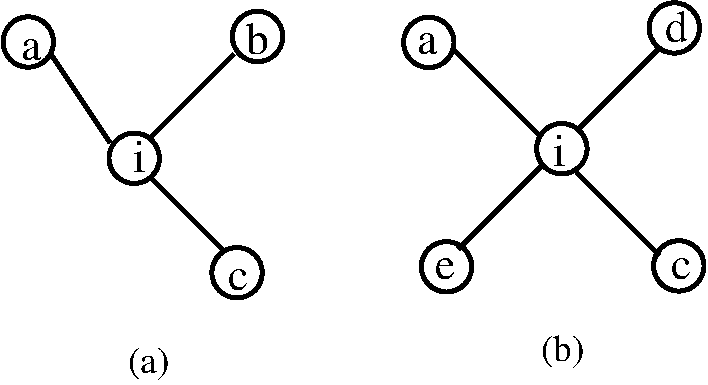
\includegraphics[width=0.45\columnwidth, angle=0]{./texfiles/Chapter_1/fig/jaccard-eps-converted-to.pdf}
 \caption{\label{fig2}(a) and (b) denote the status of node $i$ at time $t$ and $t+k$ respectively. $NBR(i)_{t}=\{a,b,c\}$ and $NBR(i)_{t+k}=\{a,d,c,e\}$ 
 $Correlation(i)_{k}$={\large$\frac{NBR(i)_{t}\bigcap NBR(i)_{t+k}}{NBR(i)_{t}\bigcup NBR(i)_{t+k}}$}={\large$\frac{2}{5}$} where $NBR(i)_{t}\rightarrow$ the set of neighbors of $i$ at time $t$}
  \end{center}
 \end{figure}
  
 \begin{figure*}
 \centering
   \includegraphics*[width=0.75\textwidth,angle=0]{./texfiles/Chapter_1/fig/age_all_5-eps-converted-to.pdf}
%    \hspace{20mm}(A)\hspace{20mm}(B)\hspace{20mm}(C)\hspace{20mm}(D)\hspace{20mm}(E)
 \caption{\label{aging}The average neighborhood-overlap value at different lags for (A)INFOCOM 2006, (B)SIGCOMM 2009, (C)Highschool 2012, (D)Highschool 2011 and (E)Hospital datasets.}
%\end{center}
 \end{figure*}

%  \begin{figure}
%  \begin{center}
%   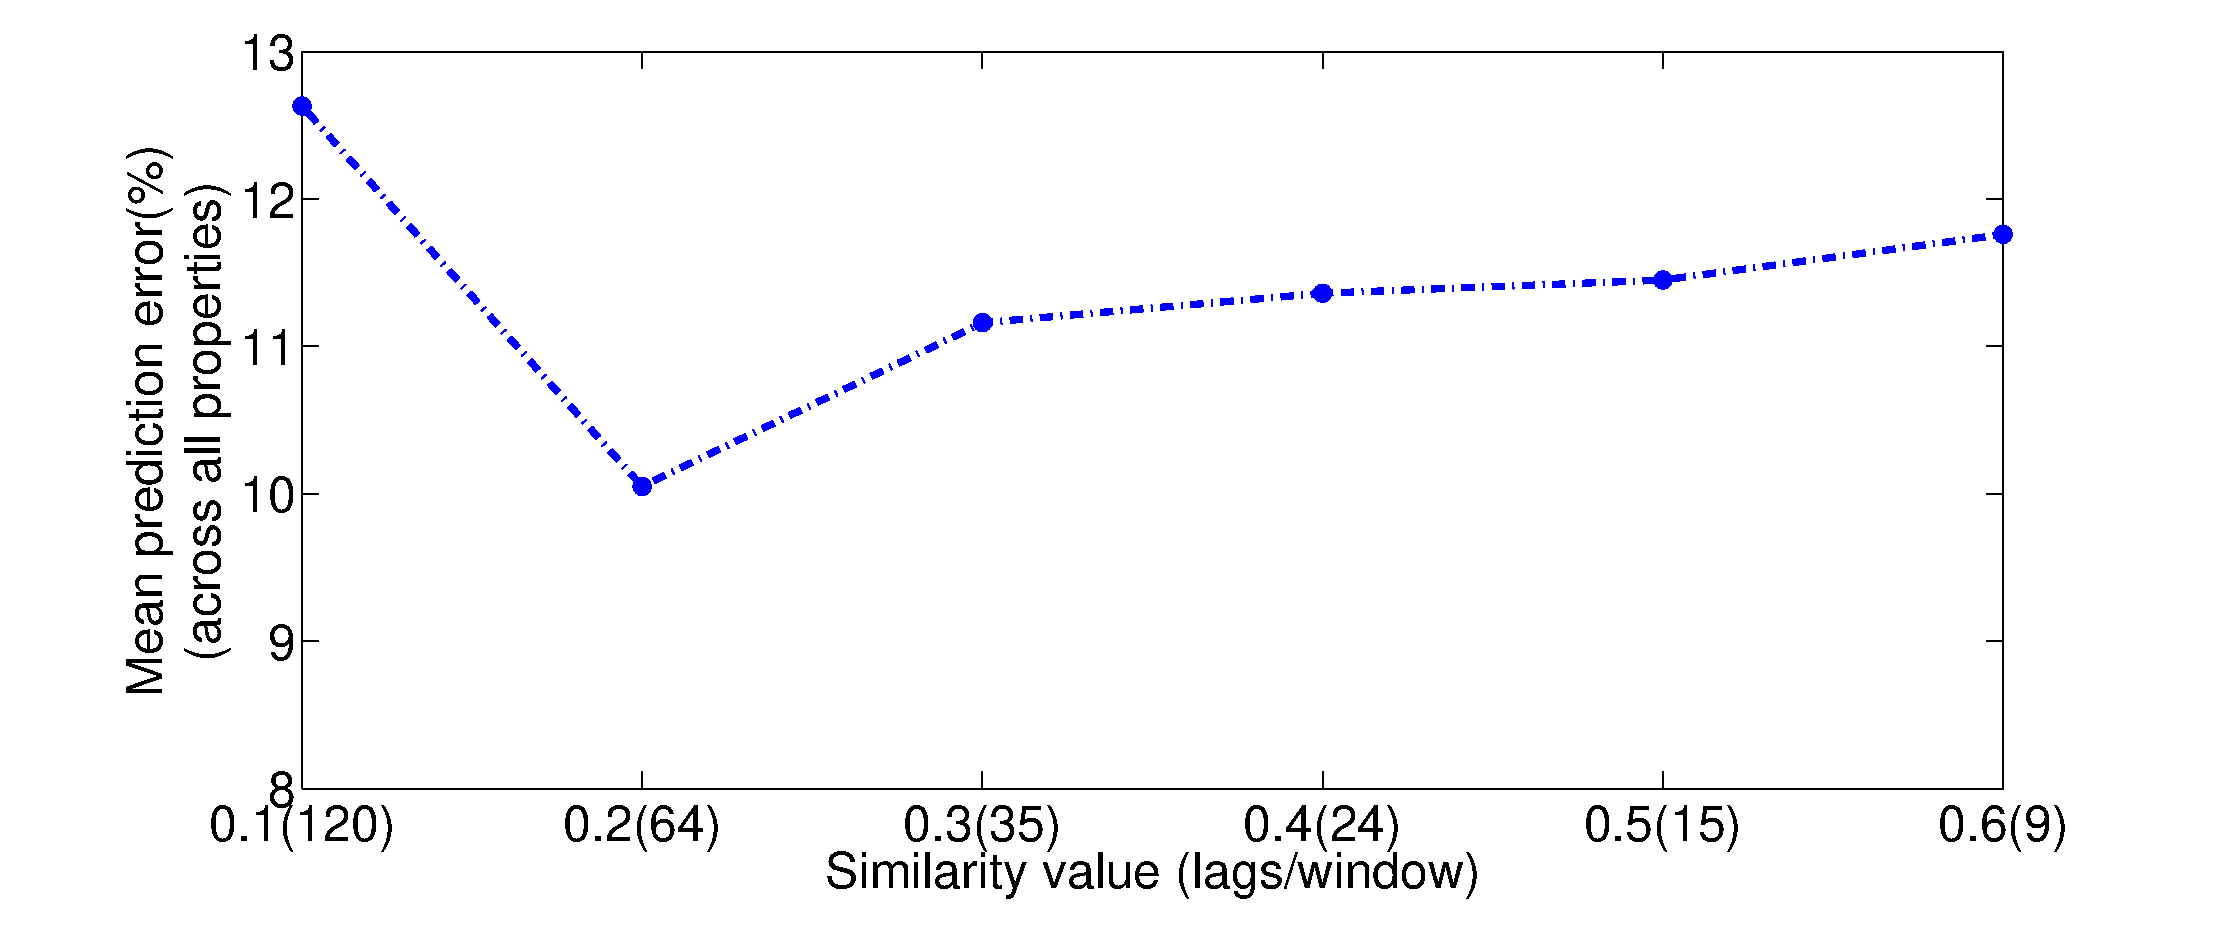
\includegraphics[width=0.75\columnwidth, angle=0]{fig/error_similarity_val.eps}
%   \caption{\label{fig_err} Mean prediction error (\%) across different properties for INFOCOM 2006 dataset for different similarity values. The lags corresponding to the similarity 
%   value are also provided.}
%   \end{center}
%  \end{figure}




% \begin{figure*}
%   \centering
%   \includegraphics*[width=0.95\textwidth,angle=0]{fig/error_dist_all.eps}
%  
%  %\hspace{8mm}(a)\hspace{60mm}(b)
%  
%  \caption{\label{fig8}  The percentage error distribution of all the properties (time series) for (A) INFOCOM 2006 dataset, (B) SIGCOMM 2009 dataset, (C) High-school 2011. (D) High-school 2012 and (E) Hospital. 
%  X-axis represents percentage error and Y-axis represents 
%  probability.}
% \end{figure*} 
  
In this section, we employ the time series to forecast the different structural properties of the temporal networks.
%Note that this process is equivalent to having a growth model for the temporal networks.
Elementary models of time series forecasting could be categorized into Auto-regressive(AR) and Moving average(MA) models ~\cite{chatfield2013analysis}. In case of 
an auto-regressive model of order $p$, AR($p$), the value of the time series at time step $t$ is given as - 
\begin{center}
 $y_{t}=\alpha_{1}y_{t-1}+\cdots+\alpha_{p}y_{t-p}+e_t+c$
\end{center}
where $\alpha_{i}$s are parameters, $e_t$ is the white noise error term and $c$ is a constant.
Similarly, in case of Moving average model of order $q$, MA($q$), the value of the time series at time step $t$ is given as - 
\begin{center}
 $y_{t}=\beta_{1}e_{t-1}+\cdots+\beta_{q}e_{t-q}+\mu+e_t+c$
\end{center}
where $\beta_{i}$s are parameters, $e_t,e_{t-1},...$ are white noise error terms and $\mu$ is the expectation of $y_t$.
These two models could be combined into Auto-regressive-moving-average (ARMA($p$,$q$)) ~\cite{chatfield2013analysis} where the value of the time series at time step $t$ is given as
\begin{center}
 $y_{t}=\alpha_{1}y_{t-1}+\cdots+\alpha_{p}y_{t-p}+\beta_{1}e_{t-1}+\cdots+\beta_{q}e_{t-q}+e_t+c$
\end{center}

However, in our case the time series show evidences of non-stationarity and short term dependencies and these models are insufficient and hence we use ARIMA model ~\cite{box2011time} for forecasting. The initial differncing step in ARIMA model 
is used to reduce the non-stationarity.
%Any ARIMA model has three parameters $p$, $d$ and $q$. $p$ is the auto-regressive element representing the lingering effects of preceding scores.
%$d$ represents the integrated element and $q$ represents the moving average element.
On fitting an ARIMA($p$,$d$,$q$) model to a time series we obtain an auto-regressive 
equation of the form-

\begin{center}
 $y_{t}=\alpha_{1}y_{t-1}+\cdots+\alpha_{p}y_{t-p}+\beta_{1}e_{t-1}+\cdots+\beta_{q}e_{t-q}+c$
\end{center}


Hence we can take a time series corresponding to a network property and fit an ARIMA model to it. Thus, we obtain an auto-regressive equation for that series which 
can be used 
in forecasting. 
% Note that our forecast results are performed on INFOCOM 2006 and SIGCOMM 2009 datasets. 
% For the Twitter hashtag co-occurrence dataset we find the time series corresponding to only some of the properties that are observed to possess a short term correlation.
% We perform our predictions only for these properties.
% For Facebook posts network also we do not perform any predictions as we find only two of the properties to be suitable for prediction. 
In order to predict a value at a future time point, we divide the data in smaller parts and perform our predictions on these smaller stretches.
In the next subsection we discuss how we perform this division.

\subsection{Selecting a window}

In order to identify the right length of a stretch (i.e., a window size) we need to identify how the network at any time point is influenced by the network at the previous time points.
The basic idea is that the time points to which this influence extends should all get included into a single window.
To quantify this influence we define a new metric called {\bf neighborhood-overlap} which measures the structural correlation between network snapshots at 
two time steps. We define the difference between these two time steps as the lag. To measure the neighborhood-overlap of the network snapshots at time 
$t$ and $t+k$, we calculate for each active node at time $t$ the overlap in its neighborhood between two time points. 
To measure this overlap we use the 
  standard Jaccard similarity as has been pointed out in ~\cite{TSMML10:smallworld}. Note that this is one of the most standard and interpretable ways to 
  measure structural similarity as has been identified in the literature with applications ranging from measuring keyword similarity ~\cite{niwattanakul2013using} to 
  similarity search in locality-sensitive-hashing (LSH) ~\cite{bawa2005lsh}. It has also been extensively used in link prediction ~\cite{lu2011link,lu2009similarity} 
  as well as community detection ~\cite{pan2010detecting}.
%\todo{Please give reference from Physics paper - prefereably EPJB}
Figure~\ref{fig2} shows how we formulate this measure using the Jaccard similarity index. We represent the neighborhood overlap at lag $k$ as the mean value 
  across all the active nodes in time step $t$. 
  To measure the extent of similarity we measure neighborhood-overlap for each snapshot at different lags and take the average of them. This essentially 
  shows, given a time specific snapshot how the similarity changes as we increase the lag. Figures ~\ref{aging}(A) - (E) show how this similarity 
  changes with time as we increase lag for the five different datasets. 
  As we increase the lag the similarity  
 decreases almost exponentially and hence considering snapshots at larger lag where the similarity value is very low could introduce error in learning the auto-regressive equation. 
 Also for a higher similarity value the corresponding lag would increasingly introduce more error in the fit due to lesser number of data points on which the ARIMA model gets trained
 to learn the fit function (see figure ~\ref{fig_err}).
 In fact we observed that the error in prediction increases if we consider a lag too small (high similarity value) or too large (low similarity value) (see figure ~\ref{fig_err}). 
 Hence we consider the similarity value of $0.2$ as the threshold for calculating the lag. For our prediction framework the corresponding value of the lag acts as 
 the window for fitting the ARIMA model.
  
  Let the size of the window be $w$ and we want to predict the value of the time series at time $t$. To our aim we consider the time series of the previous $w$ 
  time steps consisting of the values between time steps $t-1-w$ to $t-1$ and fit the ARIMA model to it and obtain its value at time step $t$. 
 We repeat this procedure for forecasting at every value of $t$. Thus, the time step $t$ is the test point and the series of points $t-w-1$ to $t-1$ form the 
  training set. One can imagine this process as a sliding window of size $w$ which is used for learning the auto-regressive equation and the point that falls immediately 
  outside the window is the unknown that is to be predicted.
  
  \begin{figure}
 \begin{center}
  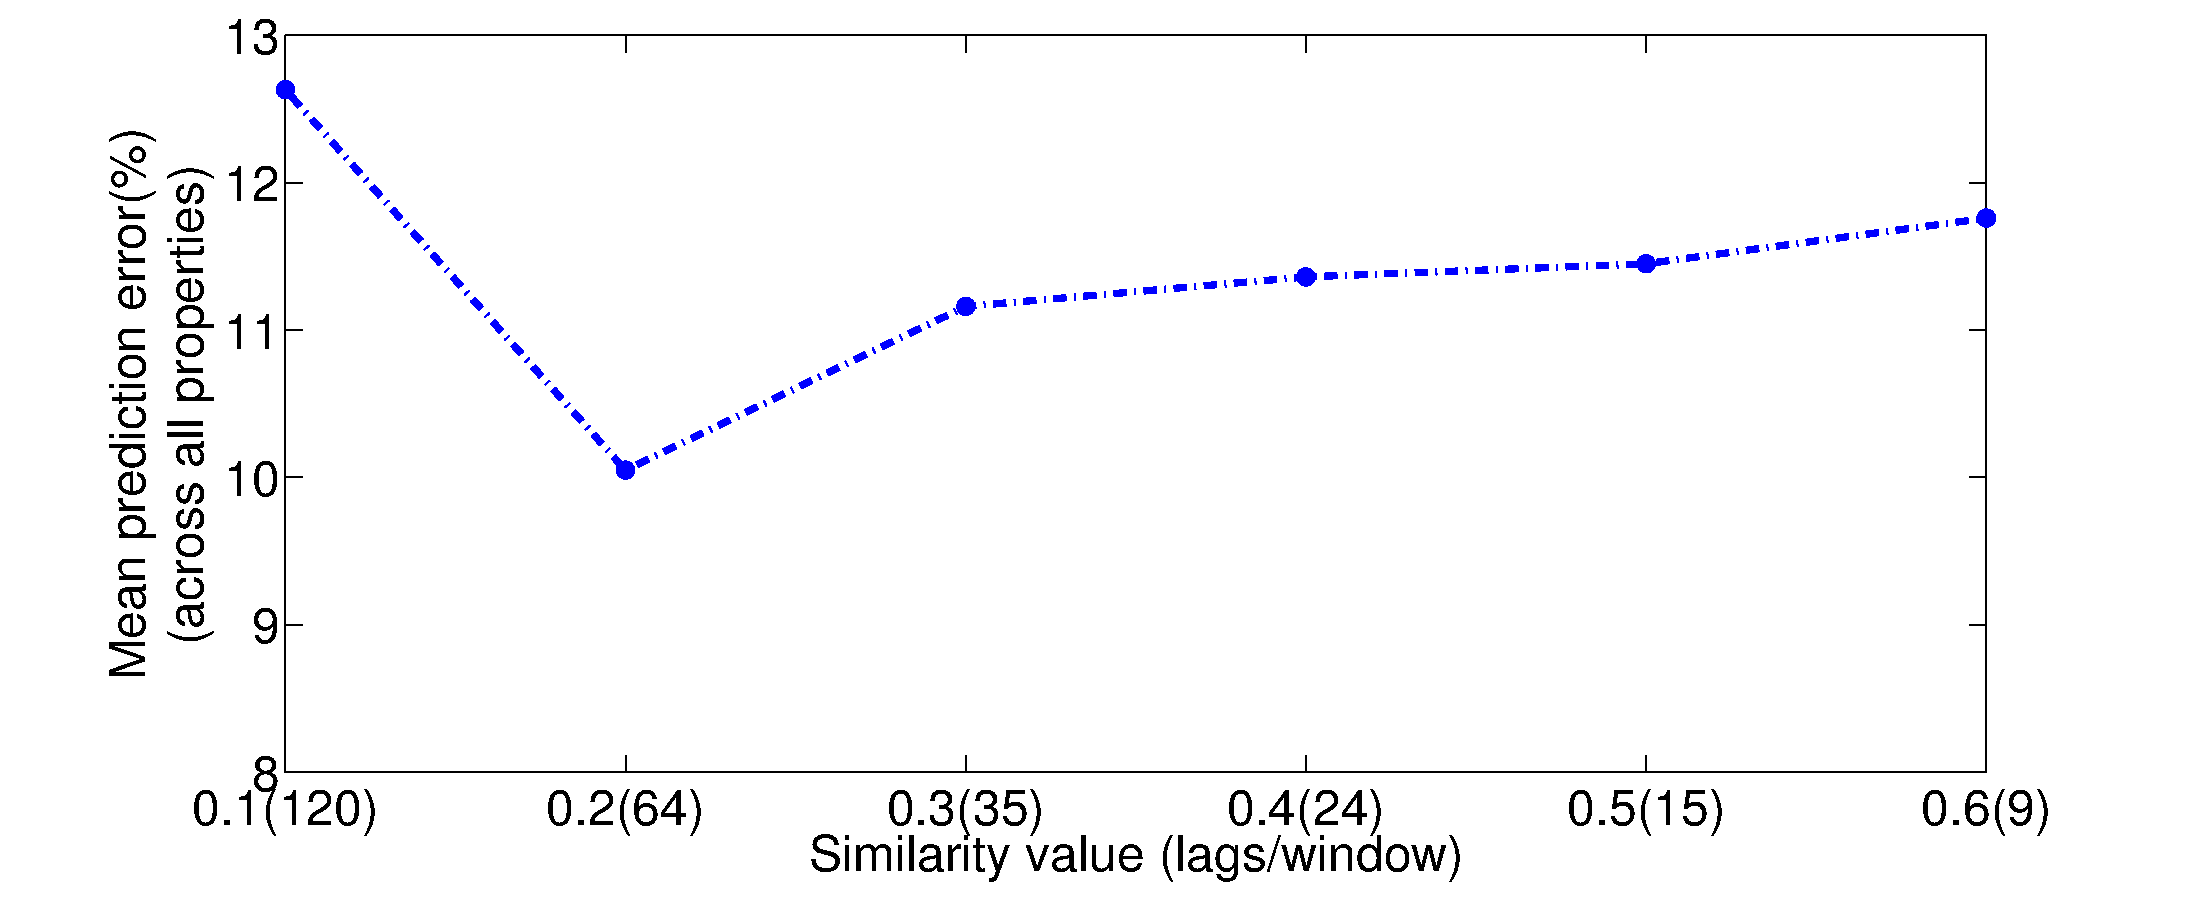
\includegraphics[width=0.75\columnwidth, angle=0]{./texfiles/Chapter_1/fig/error_similarity_val-eps-converted-to.pdf}
  \caption{\label{fig_err} Mean prediction error (\%) across different properties for INFOCOM 2006 dataset for different similarity values. The lags corresponding to the similarity 
  value are also provided.}
  \end{center}
 \end{figure}
  
  
  %   Figure ~\ref{aging} gives the value of the measure at different lags for INFOCOM 2006 dataset. To calculate the correlation value at a certain lag, we take each network snapshot 
%   and measure the average neighborhood-overlap with the snapshot at that lag and take the mean of the values.
% We observe that the value of the structural correlation decreases as we increase the lag. The correlation drops to less than 
% $0.2$ at lag around $70$.
%Therefore we select a window of size 64. 
%We could have selected any other value between 60 and 70, but we select 64 as it is in the power of 2 and it helps in the spectrogram 
%analysis we do later. 
% We observe that any choice of window size between 50 and 70 only negligibly affects the prediction outcomes. However, we set the window size to 64 since this is the 
% only poer of 2 in this admissible range and the spectrogram analysis requires that the window size to be a power of 2.
% For prediction purposes we feed the ARIMA model with the previous 64 values of the time series in order to obtain the value 
% of the current time point. 
% For the SIGCOMM 2009 dataset we perform a similar analysis and obtain a window of size 100. As it is not in the power of 2, we use a window of size 128 
% (closest integer to 100 with power of 2) for the corresponding spectrogram analysis. For the Twitter dataset we find the structural correlation to be very low 
% and it reduces even further as we increase the lag. We consider only a very small window of size 24. We do not perform spectrogram analysis for this dataset.}
% \subsection{Enhancing the prediction scheme through spectrograms}
% 
% We use spectrograms in two ways-
%  \begin{itemize}
%   \item From the spectrogram of the whole series we can determine whether this property of the network can be predicted with minimum error.
%   \item Using the local information we can determine whether a prediction at a certain time point would be erroneous or not before applying our prediction technique.
%  \end{itemize}
%  
%  We have already mentioned the presence of dominance of lower frequencies. We further observe that the extent of the dominance is 
%  an indicator whether the prediction will be appropriate or not. We describe in detail the performance of our prediction framework in the next section.
%  \begin{figure*}
%  \centering
%    \includegraphics*[width=0.75\textwidth,angle=0]{fig/age_all_5.eps}
% %    \hspace{20mm}(A)\hspace{20mm}(B)\hspace{20mm}(C)\hspace{20mm}(D)\hspace{20mm}(E)
%  \caption{\label{aging}The average neighborhood-overlap value at different lags for (A)INFOCOM 2006, (B)SIGCOMM 2009, (C)Highschool 2012, (D)Highschool 2011 and (E)Hospital datasets.}
% %\end{center}
%  \end{figure*}
% 
% 
% 
% 
% 
% \begin{figure*}
%   \centering
%   \includegraphics*[width=0.95\textwidth,angle=0]{fig/error_dist_all.eps}
%  
%  %\hspace{8mm}(a)\hspace{60mm}(b)
%  
%  \caption{\label{fig8}  The percentage error distribution of all the properties (time series) for (A) INFOCOM 2006 dataset, (B) SIGCOMM 2009 dataset, (C) High-school 2011. (D) High-school 2012 and (E) Hospital. 
%  X-axis represents percentage error and Y-axis represents 
%  probability.}
% \end{figure*}
 \begin{figure*}
  \centering
  \includegraphics*[width=0.95\textwidth,angle=0]{./texfiles/Chapter_1/fig/error_dist_all-eps-converted-to.pdf}
 
 %\hspace{8mm}(a)\hspace{60mm}(b)
 
 \caption{\label{fig8}  The percentage error distribution of all the properties (time series) for (A) INFOCOM 2006 dataset, (B) SIGCOMM 2009 dataset, (C) High-school 2011. (D) High-school 2012 and (E) Hospital. 
 X-axis represents percentage error and Y-axis represents 
 probability.}
\end{figure*} 

\medskip

 

\noindent
\section{Prediction results}
\label{result}
In this section, we provide detailed results of our prediction framework on the datasets discussed earlier.
To determine the accuracy of our prediction strategy we use the cross validation technique.  
For each time step in this range we 
use our framework to obtain a prediction at that time step. Since we already know the original value, we can obtain a percentage error for the prediction.
Let $predict_{t}$ represent the prediction value at time $t$ and $original_{t}$ represent the original value. We obtain percentage error ($error_{t}$) using the formula:
\begin{center}
 {\large$error_{t}=\frac{|original_{t}-predict_{t}|}{original_{t}}*100$}
\end{center}



First we try to find the suitable window for predicting the value of a time series at a time step. For this we refer to figure ~\ref{aging} where 
we quantify structural correlation and show how the similarity value decreases with increasing lag.
We observe that the value of the structural correlation decreases as we increase the lag. For INFOCOM 2006 dataset (figure ~\ref{aging}(A)) the correlation drops to less than 
$0.2$ at lag around $70$.
Therefore we select a window of size 64. 
Although any other value between 60 and 70 could have been selected, we opt for 64 as it is in the power of 2 and thereby helps in the spectrogram 
analysis. Similarly, we find the suitable window size to be around 128, 64, 64, 32 (closest power of 2) 
for the SIGCOMM 2009, Highschool 2011, Highschool 2012 and Hospital datasets respectively (refer to figure ~\ref{aging}). 
% If we look into the behavior in figure ~\ref{aging}(B)
%  we observe that even at lag 1 the similarity value is 0.025 and it decreases as we increase lag. We found similar behavior for Facebook posts dataset
%  as well. This essentially suggests that structural correlation does not exist in case networks representing human contact through social media. 
%  Hence we do not find a suitable window for applying our prediction framework in these networks. 
%\subsubsection{Human face-to-face interaction}
\begin{table*}
%\begin{center}
\centering
\begin{adjustbox}{max width=\textwidth}
\begin{tabular}{|c|c|c|c|c|c|}
\hline
                                                                  & \multicolumn{5}{c|}{Prediction error $\leq 20\%$}                                                                                                                                                                                                        \\ \hline
Datasets                                                          & \begin{tabular}[l]{@{}l@{}}INFOCOM \\ 2006\end{tabular} & \begin{tabular}[l]{@{}l@{}}SIGCOMM \\ 2009\end{tabular} & \begin{tabular}[c]{@{}l@{}}Highschool\\ 2012\end{tabular} & \begin{tabular}[c]{@{}l@{}}Highschool\\ 2011\end{tabular} & Hospital \\ \hline
\# Active nodes                                                   & {\bf 0.984}, (0.988)                                                  & {\bf 0.907}, (0.91)                                                   & 0.68, (0.765)                                                      & {\bf 0.861}, (0.882)                                                     & 0.782, (\underline{\it 0.859})    \\ \hline
Average degree                                                    & {\bf 0.975}, (0.968)                                                  & {\bf 0.84}, (0.834)                                                    & {\bf 0.816}, (0.81)                                                     & {\bf 0.91}, (0.908)                                                      & 0.714, (0.724)    \\ \hline
Modularity                                                        & {\bf 0.905}, (0.921)                                                  & {\bf 0.838}, (0.85)                                                   & {\bf 0.90}, (0.91)                                                      & {\bf 0.92}, (0.917)                                                      & 0.78, (0.812)     \\ \hline
Edge emergence                                                    & {\bf 0.971}, (0.983)                                                  & {\bf 0.906}, (0.91)                                                   & 0.56, (\underline{\it 0.71})                                                      & 0.42, (\underline{\it 0.512})                                                      & 0.57, (\underline{\it 0.652})     \\ \hline
\# Active edges                                                   & {\bf 0.901}, (0.91)                                                   & 0.71, (\underline{\it 0.81})                                                    & 0.72, (\underline{\it 0.78})                                                      & {\bf 0.836}, (0.86)                                                     & 0.734, (\underline{\it 0.796})    \\ \hline
\begin{tabular}[c]{@{}l@{}}Clustering \\ coefficient\end{tabular} & {\bf 0.829}, (0.858)                                                  & 0.725, (0.75)                                                   & 0.54, (\underline{\it 0.623})                                                      & 0.5, (\underline{\it 0.682})                                                       & 0.71, (\underline{\it 0.751})     \\ \hline
\begin{tabular}[c]{@{}l@{}}Closeness \\ centrality\end{tabular}   & 0.751, (\underline{\it 0.887})                                                  & 0.71, (\underline{\it 0.83})                                                    & {\bf 0.83}, (0.843)                                                      & {\bf 0.821}, (0.853)                                                     & 0.74, (\underline{\it 0.786})     \\ \hline
\begin{tabular}[c]{@{}l@{}}Betweenness\\ centrality\end{tabular}  & 0.621, (\underline{\it 0.818})                                                  & 0.472, (\underline{\it 0.61})                                                   & 0.51, (0.63)                                                      & 0.22, (\underline{\it 0.418})                                                      & 0.542, (\underline{\it 0.689})    \\ \hline
\hline
Average                                                           & 0.867, (\underline{\it 0.916})                                                  & 0.763, (\underline{\it 0.813})                                                   & 0.694, (\underline{\it 0.768})                                                     & 0.686, (\underline{\it 0.754})                                                     & 0.69, (\underline{\it 0.74})    \\ \hline
\end{tabular}
\end{adjustbox}
 \caption{\label{tab_res}Network property and the fraction of predictions with percentage error  $\leq20\%$ without (with) spectrogram analysis. 
 The cases where more than $80\%$ of the points have prediction error $\leq 20\%$ have been highlighted in bold font and the cases where on using spectrogram analysis 
 the improvement is more than $5\%$ have been underlined.}

\end{table*}
%We apply our prediction framework on (i) INFOCOM 2006 and (ii) SIGCOMM 2009 datasets.
For the INFOCOM 2006 dataset we consider the time steps 200-800. 
%We select the range from 200-800 to remove inconsistencies in the series during the initial and also towards the final stages. 
Note that selection of these is only representative and one is free to take 
any time step, subject to the condition that a window of appropriate length is available. For SIGCOMM 2009, High School 2012, Highschool 2011 and Hospital datasets we 
consider our test time steps to be 300-900, 200-1000, 200-1000 and 100-900 respectively (refer to table 1). 
% for Twitter hashtag co-occurrence dataset we consider the time steps 100-600.
%  We do not apply our prediction framework for the Facebook posts data.
% For each time step in this range we 
% use our framework to obtain a prediction at that time step. Since we already know the original value, we can obtain a percentage error for the prediction.
% Let $predict_{t}$ represent the prediction value at time $t$ and $original_{t}$ represent the original value. We obtain percentage error ($error_{t}$) using the formula:
% \begin{center}
%  {\large$error_{t}=\frac{|original_{t}-predict_{t}|}{original_{t}}*100$}
% \end{center}


%-eps-converted-to.pdf
\begin{figure}
 \begin{center}
 \includegraphics[width=0.89\columnwidth, angle=0]{./texfiles/Chapter_1/fig/psd_pred-eps-converted-to.pdf}
 \caption{\label{k1}(A) LPSD versus mean percentage error for all the properties across all the datasets.}
  \end{center}
 \end{figure}


  
%\todo{Is Fig 8 a new figure}
 

%\todo{This para is very poorly written}
To check how efficient our predictions are we plot the cumulative probability distribution of percentage error for all the datasets in figure ~\ref{fig8}. 
In table ~\ref{tab_res}, we compare the prediction results across different datasets and different metrics for cases where the prediction error $\leq20\%$. 
 Note that this error level is representative and ideally a table can be recovered for each such error level from figure ~\ref{fig8}. We make the 
 following observations from the results: 
\begin{itemize}
 \item  Our framework is able to predict the values for active nodes, average degree and modularity with high accuracy across all datasets. 
%  In fact the prediction error is 
%  less than or equal to $20\%$ with probability 0.84, 0.85 and 0.86 respectively for active nodes, average degree and modularity on an average across all datasets.
 \item For active edges, edge emergence, clustering coefficient and closeness centrality, our framework is able to predict the values with moderate accuracy although the 
 prediction accuracy for these properties is reasonably high for some datasets (INFOCOM 2006, SIGCOMM 2009).
 \item The prediction accuracy is poor across all datasets for betweenness centrality and in some cases for clustering coefficient and closeness centrality.
\end{itemize}


An important observation is that the spectrogram analysis (introduced in section ~\ref{properties}) is able to distinguish between these properties based on their 
 predictability. On ranking the properties based on the PSD value at bin 1 (refer to figures ~\ref{fig_all_dataset}(B), (D), (F) and ~\ref{fig_all_dataset_1}(B), (D)), we observe 
 that the higher ranked properties are the ones for which the prediction error is low while the lower ranked ones have higher prediction error. 
 Following this observation we further plot the mean percentage error for all the properties across all the datasets versus LPSD in figure ~\ref{k1}. 
 The plot clearly shows that the higher the value of LPSD, lower is the 
mean percentage of error and vice versa.
%This shows that spectrogram of the time series can be used to determine whether a property can be predicted with low percentage error in prediction.

On further investigating into the cases where the prediction error is high, we observe that these points are mostly located either in places where a sharp 
 transition occurs or in silent phases where there is limited interaction among the nodes. Figure~\ref{fig9} identifies some of the transition and silent phases 
 in the time series of the number of active edges in INFOCOM 2006 dataset.
Similar phases are also present in the other datasets as well. 
 %An immediate extension to check whether we can leverage spectrogram analysis to identify these points beforehand. 
%  To our aim we extend the spectrogram analysis to the single point case whereby  
%  while predicting a property at a give time step, we find that the spectrogram of the window ($w$) and use the LPSD value as an indicator for prediction accuracy. 
% We 

 \begin{figure}[!ht]
  \begin{center}
  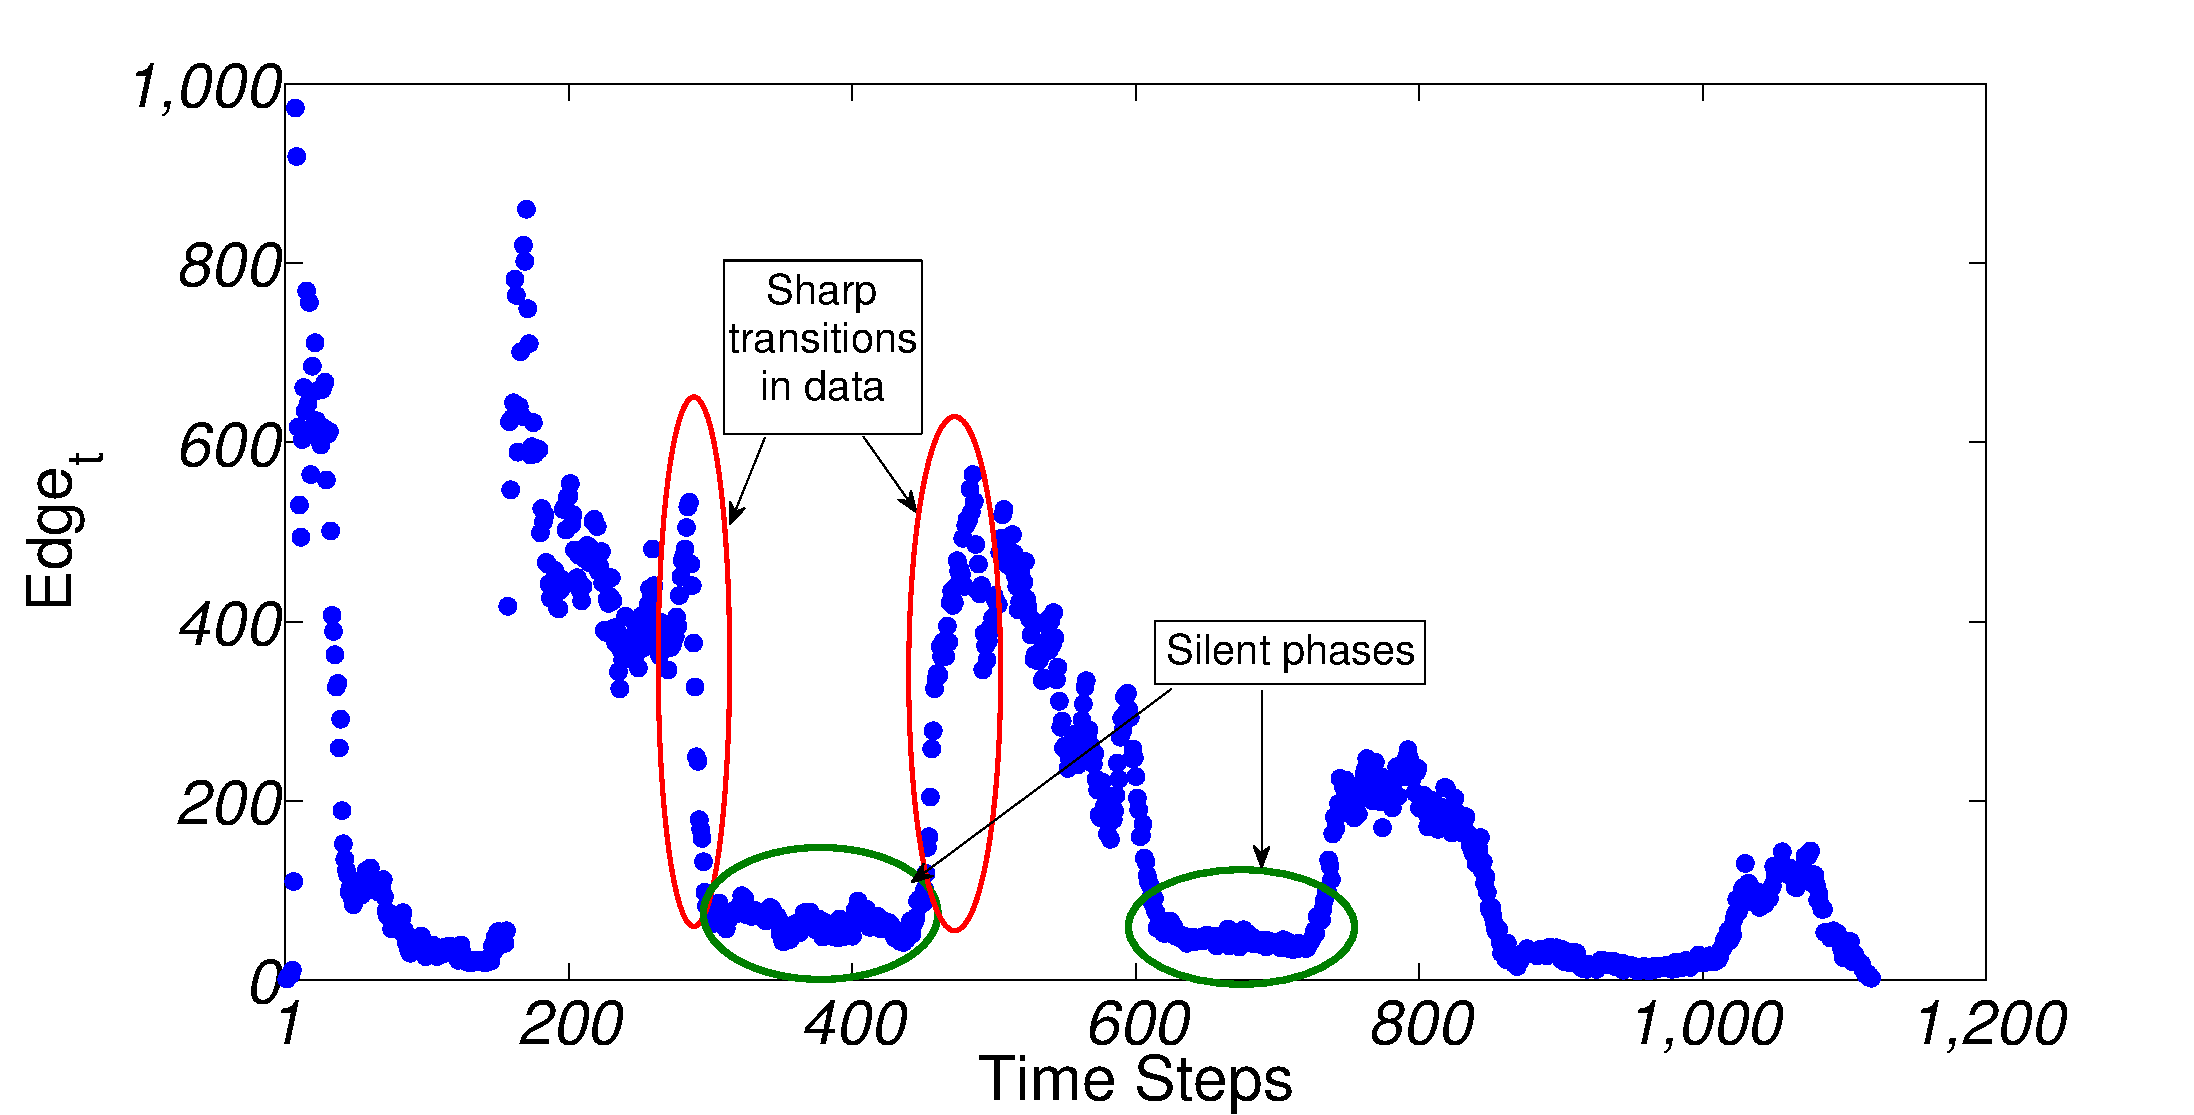
\includegraphics[width=0.7\columnwidth, angle=0]{./texfiles/Chapter_1/fig/no_of_edges1-eps-converted-to.pdf}
  \caption{\label{fig9}The time series plot for number of active edges. The red and the green ellipses identify
  two transition and two silent phases respectively}
  \end{center}
 \end{figure}

%  \begin{figure}
%  \begin{center}
%  \includegraphics[width=0.89\columnwidth, angle=0]{fig/psd_pred-eps-converted-to.pdf}
%  \caption{\label{k1}(A) LPSD versus mean percentage error for all the properties across all the datasets.}
%   \end{center}
%  \end{figure}
%\todo{Make Fig 10 more square -- otherwise difficult to understand}
 
 \begin{figure}[!ht]
  \begin{center}
  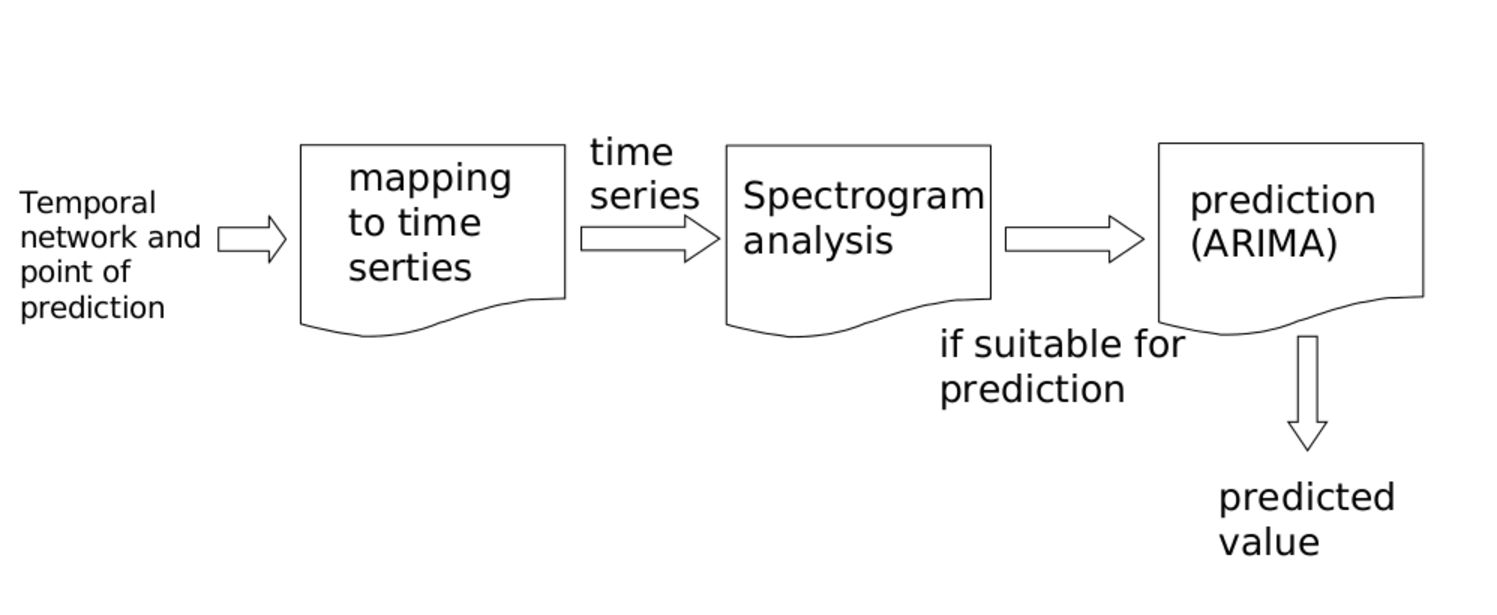
\includegraphics[width=0.95\columnwidth, angle=0]{./texfiles/Chapter_1/fig/Prediction.pdf}
  \caption{\label{fig:e_pred}The prediction framework.}
  \end{center}
 \end{figure}


%\subsection{Capturing the high error points}
%We next concentrate on the time points where the prediction error is high. 
% For the 600 time steps we considered, only in case of 8 time points for INFOCOM 2006 dataset and 32 time points in case of SIGCOMM 2009 dataset, did we find 
% more than five of the eight properties to give prediction error percentage more than 20\%. 
% \textcolor{blue}{Once again the error level chosen is representative and similar results are obtained for 10\% and 30\% error levels.} 
% For High school 2012, High school 2011 and Hospital datasets the corresponding 
% numbers are 42, 38 and 52 respectively.
% We observe that these points are mostly located either in places where a sharp transition occurred or in silent phases where there was limited interaction among the nodes.
% % On further 
% % investigation we find them to be either in places where a sharp transition has occurred or in the silent phases where there are have been limited interaction among the nodes.
% Figure~\ref{fig9} identifies some of the transition and silent phases in the time series of number of active edges in INFOCOM 2006 dataset.
% Similar phases are also present in the other datasets as well. 
% Next we check whether we can identify these points beforehand.
% These transition phases or silent phases are the idiosyncrasies of the dataset. 
% Since we are using human communication network, transition phases occur mostly due to the bursty nature of the network.
% We believe that our strategy will give even better result for datasets with higher stationarity. 
\begin{figure*}[!ht]
  \begin{center}
  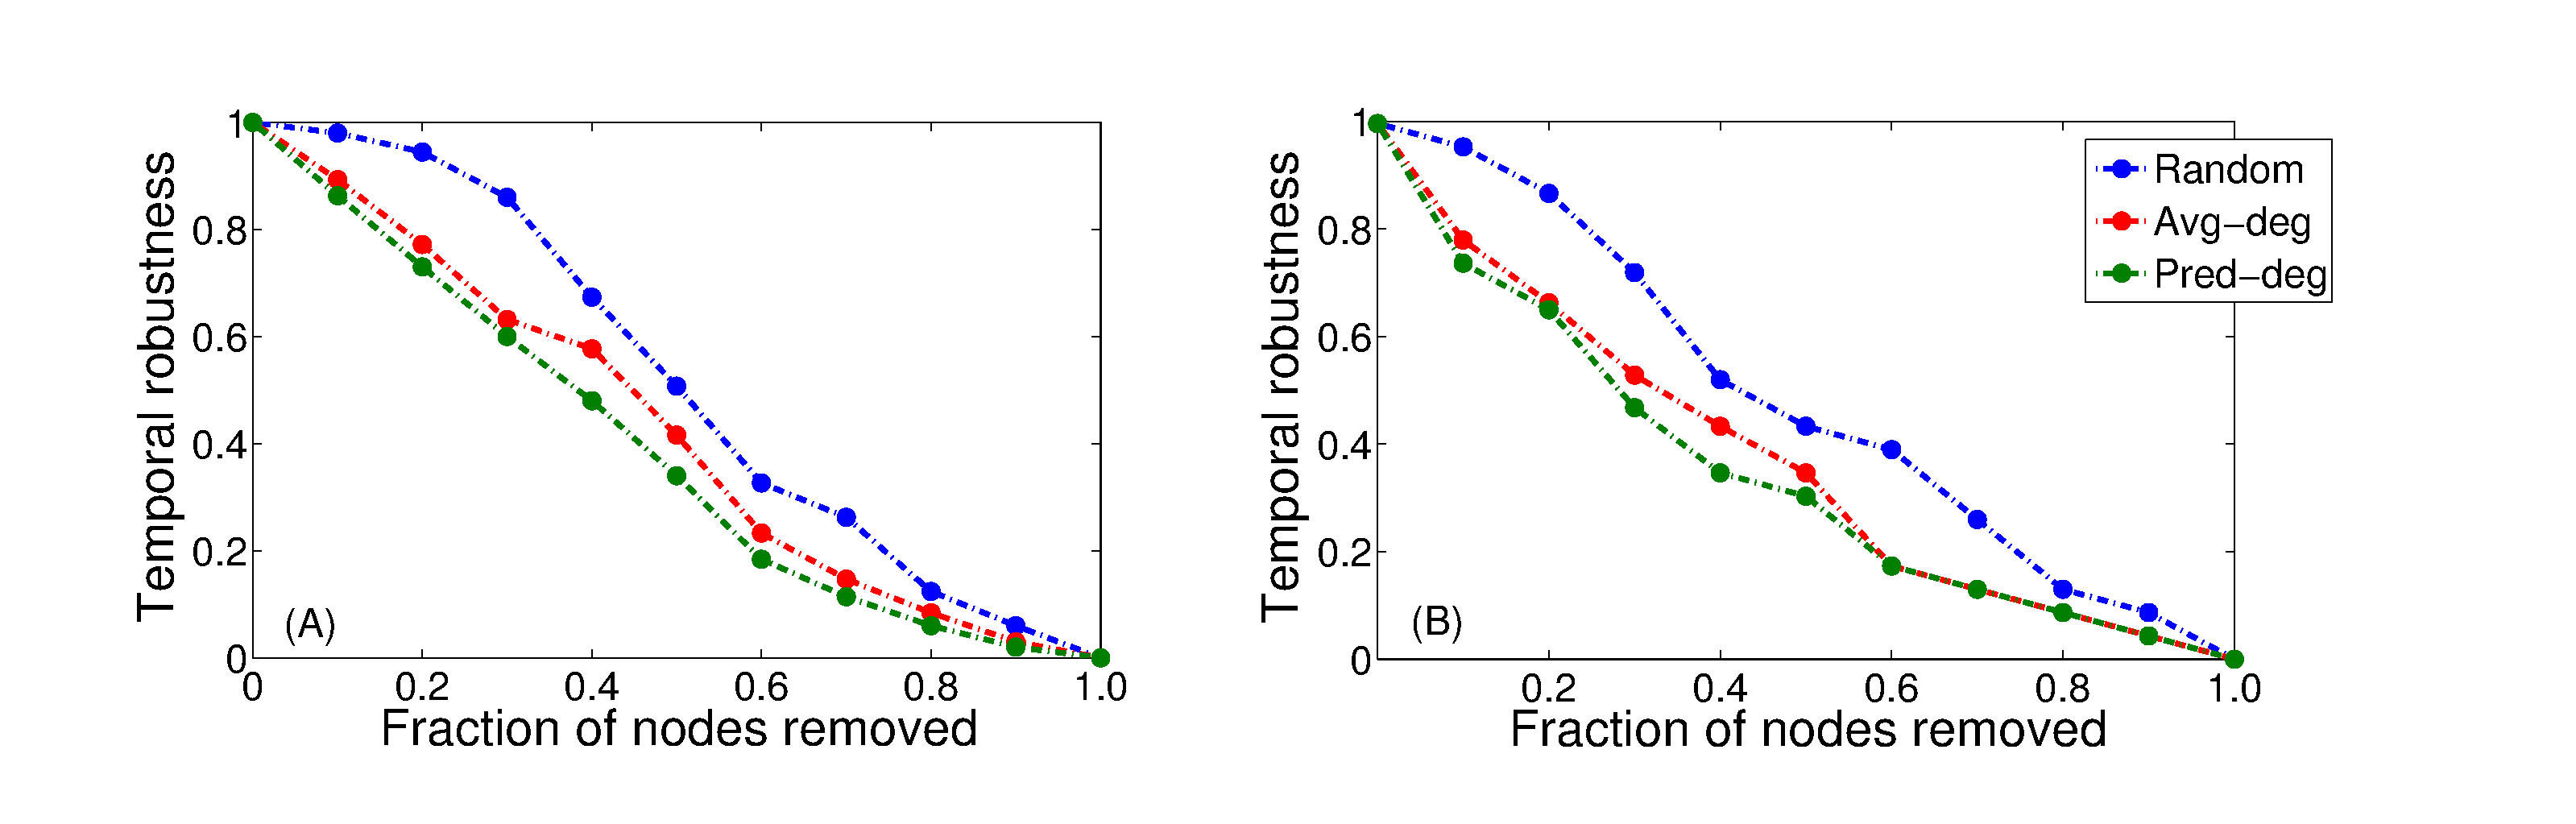
\includegraphics[width=0.9\linewidth, angle=0]{./texfiles/Chapter_1/fig/attack_all-eps-converted-to.pdf}
  \caption{\label{fig_attack}Temporal robustness as a function of the fraction of removed nodes for (a) INFOCOM 2006 and (b) SIGCOMM 2009 datasets.}
  \end{center}
 \end{figure*}

 
% Previously we have seen that spectrogram analysis on the time series of the properties is able to separate out the properties which are predictable (low errors in prediction). 
% We further plot the 
% mean percentage error against the mean PSD of frequencies $<$ 5 Hz (bin 1) in figure ~\ref{k1}(A). The plot clearly shows that the higher the value LPSD lower is the 
% mean percentage error and vice versa. Thus through the spectrogram of the time series we can conclude whether a property can be predicted 
% with low percentage error in prediction.
% To check whether the prediction at a time point would be erroneous, we extend the spectrogram analysis to the single point case. 
% While predicting a property at a give time step, we find that the spectrogram of the window ($w$) can be an 
% indicator for prediction accuracy. To our aim we consider two time steps: one where the prediction error is low and other where it is high for the property 
% number of active edges (INFOCOM 2006 dataset).
% In figure ~\ref{k1}(B) we plot the corresponding mean PSD value for the frequencies $<$ 5 Hz (bin 1) 
% for the two time steps. We observe 
% that the mean PSD value corresponding to the frequencies $<$ 5 Hz (bin 1) to be much higher in case where the prediction error is low (1) than 
% in the case where the prediction error was high (2). In fact this method could identify most of the points which where present in the transition or silent phase. 
% All these observations lead us to believe that spectrogram analysis can be used to filter out cases where the prediction error is high and thereby improve 
% the overall accuracy of our prediction framework.
 
 
 
\subsection{Enhancing the prediction scheme through spectrogram}

Since spectrogram analysis of the time series could determine the predictability of the corresponding property, 
an immediate extension would be to check whether it could be leveraged to identify beforehand the cases where the prediction error is high (unsuitable for prediction). 
To that aim we extend the spectrogram analysis to the single point case whereby  
 while predicting a property at a give time step, we find that the spectrogram of the window ($w$) and use the LPSD value as an indicator for potential prediction accuracy. 
 The cases identified by spectrogram analysis to be unsuitable for prediction can then be filtered out to improve the overall accuracy of the prediction framework. 
  A schematic diagram of this enhanced prediction framework is 
 provided in figure ~\ref{fig:e_pred}.
We now consider all the datasets and the corresponding time steps for prediction (which we considered earlier in this section, refer to table 3.1) and  
instead of directly using our prediction framework we 
 perform spectrogram analysis (single point method) on these points to separate out those which are unsuitable for prediction. We predict 
 only the points which the spectrogram analysis identifies as suitable for prediction.
 In table ~\ref{tab_res} we compare the fraction of predictions with 
 error $\leq 20\%$ between both the cases where we do not use spectrogram  and where we make use of it. 
 We observe that the fraction of prediction with error $\leq 20\%$ is enhanced for all the properties, albeit only marginally in some cases where the accuracy has already been high. 
 More importantly, for (ill-predicted) properties like betweenness centrality, closeness centrality, the prediction
accuracy increases substantially. 
 Note that prediction error $20\%$ is again representative and similar results 
 could be obtained for other values of prediction error as well.

% \subsubsection{Human interaction through social media}
% 
% \textcolor{blue}{We also applied our framework for the Twitter hashtag co-occurrence (London olympics) dataset for the properties for which short term correlation was present.
% We fixed the range of time steps between 100 and 600 and the average value of the fraction of predictions with percentage error less than or equal to 20\% 
% is 0.48. In table ~\ref{tab_twt} we report the detailed results. 
% As mentioned earlier we donot apply our prediction framework on the Facebook posts dataset.}
% 
% \begin{table}[h]
% \begin{tabular}{|c|c|c|c|c|c|c|}
% \hline
% \multirow{2}{*}{Network features} & \multicolumn{6}{l|}{Percentage error}                                     \\ \cline{2-7} 
%                                   & \multicolumn{3}{l|}{\textless=10\%} & \multicolumn{3}{l|}{\textless=20\%} \\ \hline
% Number of active nodes            & \multicolumn{3}{l|}{0.33}           & \multicolumn{3}{l|}{0.551}           \\ \hline
% Number of active edges            & \multicolumn{3}{l|}{0.294}          & \multicolumn{3}{l|}{0.494}           \\ \hline
% Average degree                    & \multicolumn{3}{l|}{0.276}          & \multicolumn{3}{l|}{0.517}          \\ \hline
% Clustering coefficient            & \multicolumn{3}{l|}{0.216}          & \multicolumn{3}{l|}{0.401}               \\ \hline
% Average            & \multicolumn{3}{l|}{0.275}          & \multicolumn{3}{l|}{0.485}               \\ \hline
% \end{tabular}
% \caption{\label{tab_twt}Network property and the fraction of predictions with percentage error less than or equal to 10\% and 20\% for Twitter hastag co-occurrence 
% network.}
% \end{table}

\medskip


\noindent
% \begin{figure*}[!ht]
%   \begin{center}
%   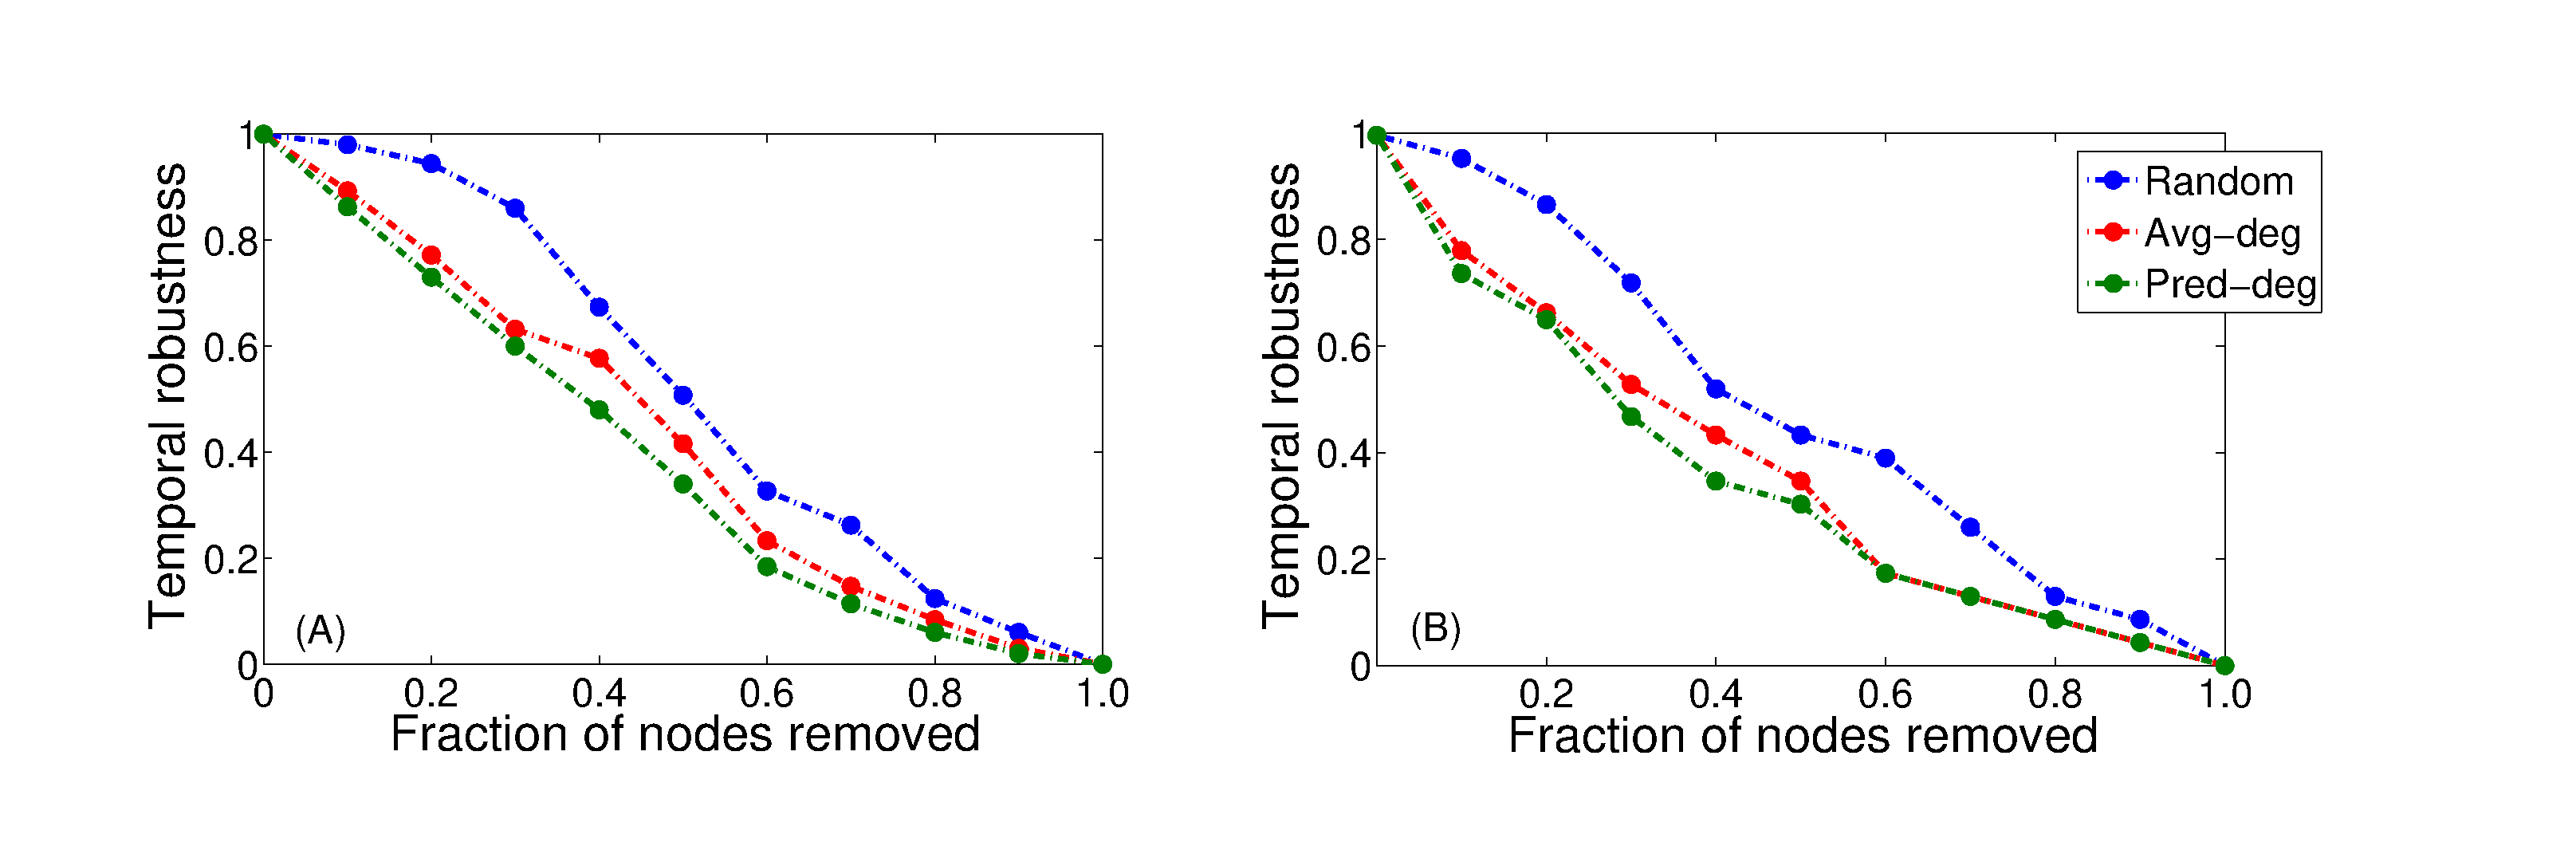
\includegraphics[width=0.9\linewidth, angle=0]{fig/attack_all.eps}
%   \caption{\label{fig_attack}Temporal robustness as a function of the fraction of removed nodes for (a) INFOCOM 2006 and (b) SIGCOMM 2009 datasets.}
%   \end{center}
%  \end{figure*}

\section{An attack strategy using prediction framework}
\label{attack}
%\todo{Be careful to have the window size `w' to be same for all the techniques -- I think thisis not there}
In this section we show how our prediction can be used in order to launch targeted attack on temporal networks. The strategy proposed is a modification over the average node degree attack presented in ~\cite{trajanovski2012error}. 
In case of average node degree attack the temporal degree\footnote{Given a time interval [$t_1, t_n$] temporal degree of node $i$ is the average degree of $i$ over the time interval}  
~\cite{trajanovski2012error} of the nodes are calculated and the node with highest temporal degree is removed in the 
subsequent steps (i.e., ``the node is attacked''). 
We observe that for every 
node its degree over a given time interval forms a time series. Using our prediction framework we calculate the degree of the node at a future time step based on the previous 
$w$ time steps (window size for the corresponding dataset, refer to section \ref{prediction})
and remove a node with the 
highest degree as predicted by our proposed framework. We compare our strategy (Pred-deg) with average node degree based attack (Avg-deg) and the random case (nodes are selected at random 
and removed). 
The effectiveness of an attack strategy is measured using temporal robustness ~\cite{trajanovski2012error} which is estimated by the relative change in efficiency ~\cite{trajanovski2012error} 
after a structural damage $D$. 
Temporal efficiency of a network $G$ in a given time interval [$t_1,t_n$], $E_G(t_1,t_2)$ is defined as the averaged sum of the inverse temporal distances over all pairs of 
nodes in that time interval. 
\begin{center}
 $E_G(t_1,t_2)=\frac{1}{N(N-1)}\Sigma_{i,j:i\neq j}\frac{1}{d_{ij}(t_1,t_2)}$
\end{center}
Here $N$ is the number of nodes in the network and $d_{ij}(t_1,t_2)$ is the temporal distance which is the smallest temporal length paths among all the temporal
paths between $i$ and $j$ in the time interval [$t_1,t_2$]. Hence, temporal robustness is defined  as $R_G(D)=\frac{E_{GD}}{E_G}$. 
In figure~\ref{fig_attack} we plot temporal robustness 
as a function of the fraction of nodes ($P$) removed 
for (a) INFOCOM 2006 and (b) SIGCOMM 2009 datasets. 
We observe that our strategy 
does better than both the random and average node degree based strategy. 

\if{0}
The reason for this result is straightforward. In the original average node degree based attack one averages 
the degree of a node for $n$ previous time steps and uses the value to rank the nodes of the $(n+1)^{st}$ time step (test data) and removes the top $P$ fraction of nodes. 
In our method, we use the actual degree values of the previous $n$ steps (training data), visualize them as a time series and predict the degree values of the $(n+1)^{st}$ step. The scheme based on 
the predicted degree values (which are pretty accurate estimates of the actual degree values of the $(n+1)^{st}$) is expected to produce a better ranking than the state-of-the-art 
scheme. As an additional advantage spectrogram analysis can also separate out the cases where our strategy would not work. 
Note that similar attack strategies could be developed based on other network properties as well.
We believe that our framework can be used as a better ranking scheme for nodes in a temporal network at a future time instant even if the network structure itself at that time point 
is unknown.
% \begin{figure*}[!ht]
%   \begin{center}
%   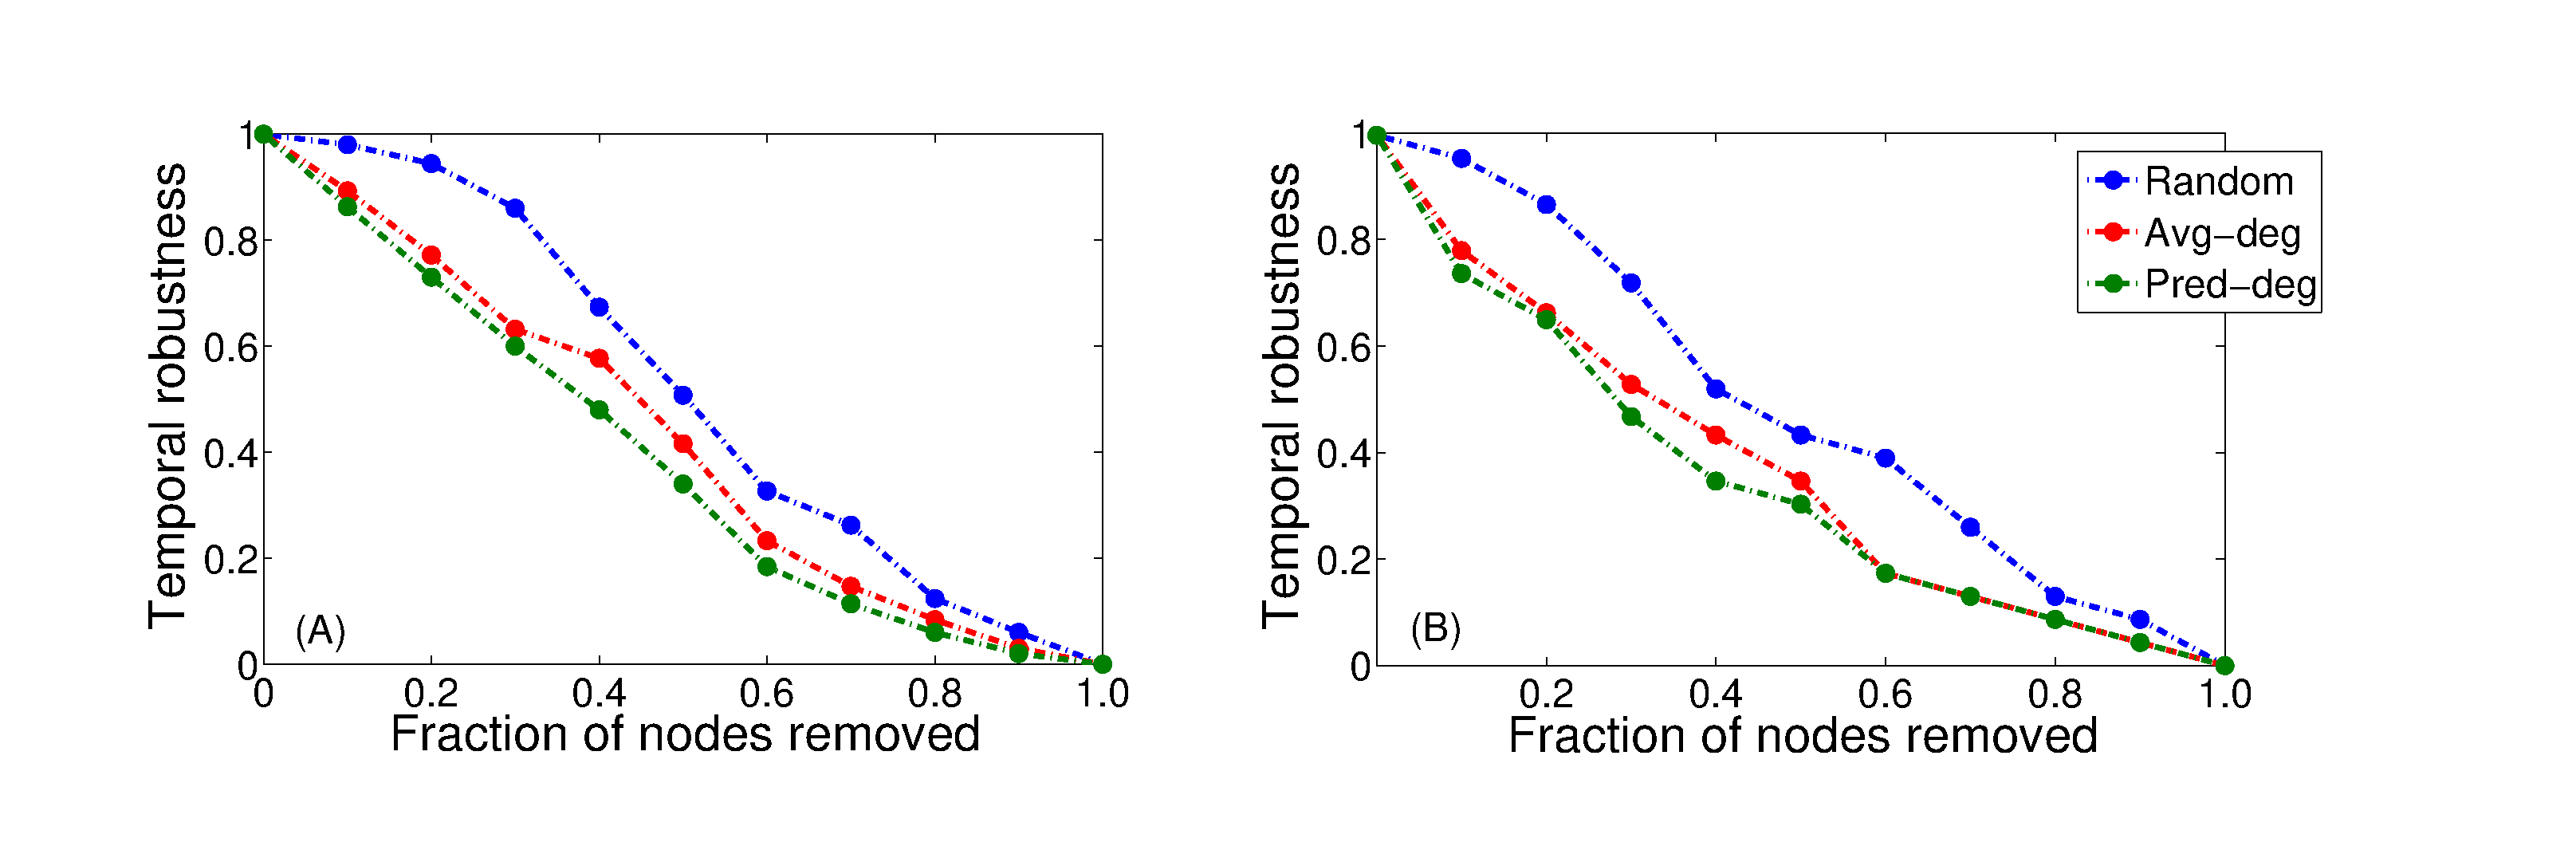
\includegraphics[width=0.9\columnwidth, angle=0]{fig/attack_all.eps}
%   \caption{\label{fig_attack}Temporal robustness as a function of the fraction of removed nodes for (a) INFOCOM 2006 and (b) SIGCOMM 2009 datasets.}
%   \end{center}
%  \end{figure*}
\fi


% \todo{This section is not needed -- remove}
% \subsection{Insights}  
% \label{insights}
% %\textcolor{blue}{
% \begin{itemize}
% %  \item Based on our analysis we can conclude that temporals networks representing human interactions can be sub divided into a two different classes. The datasets INFOCOM 2006 and 
% %  SIGCOMM 2009 which represent human face-to-face interaction differ significantly from the Twitter hashtag co-occurrence and the Facebook posts dataset 
% %  which represent human communication through social media. 
% %  Unlike the previous cases the 
% %  Twitter hashtag co-occurrence network is memory-less and almost no structural correlation exists. 
% %  For Facebook posts network also we find the network to be memory-less with only few of the properties showing presence of auto-correlation.
%  %From our analysis we are able to identify more than one class of temporal networks (we identify at least two here) and also conclude that not all temporal networks show structural 
%  %correlation.
%  \item 
% \todo{ Something like this may come just after prediction - I have diccussed with SS}
% We observe that the structural properties of a temporal network can be classified based on how well they can be predicted. We further observe that for 
%  both the datasets edge-emergence and number of active nodes give the best prediction result while betweenness centrality offers the worst prediction result.
%   This can be attributed to the fact that 
%  a person (node) who is a part of a conversation (network) at a time instant will remain a part of it in the next few time instances with high probability.
%  However, the node being a part of many shortest paths is a far rare event. 
% \todo{If you want you can mention it passingly in the conclusion}
%  \item In its current state our framework can predict the values of the network properties at a future time step but is unable to offer the exact network 
%  structure at that time step. But our framework can have genuine contributions toward link prediction in temporal networks. Since we show that structural 
%  correlation exists in these networks and we can also predict the network properties at these time steps as well, we can re-frame the link prediction problem 
%  as a network at a time step which is obtained from the network at a previous time step with minimal changes made depending on the values of the properties. 
%  We plan to deeply investigate this problem in subsequent works.
% \end{itemize}
% %}

% \subsection{An attack strategy using prediction framework}
% In this section we propose an attack strategy using based on our prediction framework. The strategy proposed is a modification over the average node degree attack. In case 
% of average node degree attack the temporal degree ~\cite{trajanovski2012error} of the nodes are calculated and node with highest temporal degree is attacked. We observe that given a 
% node its degree over a given time interval forms a time series. Using our prediction frame work we calculate the degree of the node at a future time step and remove a node with the 
% highest degree as obtained from the frame work. We compare out strategy (Pred-deg) with average node degree based attack (Avg-deg) and the random case (nodes are selected at random 
% and removed). In figure ~\ref{fig_attack} we plot temporal robustness ~\cite{trajanovski2012error} as a function of the fraction of nodes removed for Infocom 2006 dataset. We observe that our strategy 
% does better than both the random and average node degree based strategy. Note that similar attack strategies could be developed based on other network properties as well.
% 
% \begin{figure}[!ht]
%   \begin{center}
%   \includegraphics[width=0.7\columnwidth, angle=0]{fig/attack.eps}
%   \caption{\label{fig_attack}Temporal robustness as a function of the fraction of removed nodes for Infocom 2006 dataset.}
%   \end{center}
%  \end{figure}


\medskip


\noindent
\section{Summary of this chapter}
\label{conclusion}

Our contributions in this chapter can be summarized as below:
\begin{itemize}

\item we provided a general framework to map temporal network of human contacts consisting of a series of graphlets equispaced in time into time series
and provide a detailed time domain and frequency domain analysis.

\item we re-established the presence of structural correlation in a temporal network of human face-to-face contact using a new metric which we call
neighborhood-overlap.

\item we further quantified the extent of this correlation using neighborhood-overlap and used it to identify the correct window size in our prediction framework.

\item we also provided an approach for predicting the properties of future network instances using time series as a proxy and showed that even though the 
precise network structure is not known at time step, one can estimate its properties.

\item finally, we provided a frequency domain analysis of temporal network and leveraged it to enhance the prediction accuracy.

\item as an application we showed how our framework could be used in devising better strategies for targeted network attacks.
 
 \end{itemize}
 
 In its current state our framework can predict the values of the network properties at a future time step but is unable to offer the exact network 
 structure at that time step. But our framework can have genuine contributions toward link prediction in temporal networks. Since we show that structural 
 correlation exists in these networks and we can also predict the network properties at these time steps as well, we can re-frame the link prediction problem 
 as a network at a time step which is obtained from the network at a previous time step with minimal changes made depending on the values of the properties. 


\medskip

% \bibliographystyle{unsrt}


%\bibliography{ref}



%\end{document}

% end of file template.tex

